\documentclass[11pt,letterpaper]{article}
\usepackage[utf8]{inputenc}
\usepackage[sc]{mathpazo}

\usepackage[T1]{fontenc}
\usepackage{amsmath}
\usepackage{amsfonts}
\usepackage{amssymb}
\usepackage{graphicx}
\usepackage{comment}
\usepackage{bbm}
\usepackage{hyperref}
\usepackage{apacite}
\usepackage{natbib}
\usepackage{har2nat}
\usepackage[width=16.00cm, height=23.00cm]{geometry}
\usepackage{tablefootnote}
\usepackage{multirow}
\usepackage{longtable}
\usepackage{rotating, tabularx}
\usepackage{booktabs}
\usepackage{threeparttable}
\usepackage[table,xcdraw]{xcolor}
\usepackage[dvips]{xcolor}
\usepackage{pdflscape, lipsum}
\usepackage{tabularx}
\usepackage{url}
\usepackage{float}
\usepackage[capposition=top]{floatrow}
\usepackage{subcaption}

%\usepackage{hyperref, cleveref}
\usepackage{xr}
\externaldocument{MPHI_Appendix}
\usepackage[toc,page]{appendix}


\definecolorseries

\usepackage[pagewise]{lineno}
%\linenumbers

\renewcommand{\baselinestretch}{1.3}
%\linespread{1.3}         % Palladio needs more leading (space between lines)


\hypersetup{colorlinks,linkcolor={[rgb]0.7, 0.11, 0.11},citecolor={[rgb]0.7, 0.11, 0.11}, filecolor={[rgb]0.7, 0.11, 0.11}, urlcolor={[rgb]0.7, 0.11, 0.11}}  
%magenta
%\hypersetup{colorlinks=false, urlbordercolor=blue}
%0,0.88502,1,0
\usepackage{booktabs,siunitx,amsmath,caption}

%-------------------------------------------------------------------
\author{Kosal Nith\footnote{Email: \href{mailto:nithkosal@futureforum.asia}{\texttt{nithkosal@futureforum.asia}}. Webpage: \url{https://nithkosal.github.io}.} \\
	\small{Future Forum}  
}

\title{\textbf{Monetary Policy and Household Income Distribution: An Empirical Analysis from Cambodia\footnote{I cannot find enough words to thank my friend Phay Thounimith for his usual meeting in dicusse and help almost every weekend. I have particularly benefited from the comments of Ou Virak, and Adrien Auclert. I also thank the National Institute of Statistics for offering the dataset, in particular, Nor Vanndy for coordinating to provide the CSES dataset, Michele Piffer for sharing the replication codes of the Romer shocks.}}}
%-------------------------------------------------------------------
\begin{document}
	

	 %PRELIMINARY AND INCOMPLETE 
	 
%-------------------------------------------------------------------	  
\maketitle
	\begin{abstract}
	This paper investigates to estimate the distributional effects of monetary policy shocks on macroeconomic aggregates and aggregate consumption. An earning heterogeneity channel, a Fisher channel and an interest rate exposure channel were applied as transmission channels affect aggregate spending when households have different average propensities of consume. Through the Structural VAR model, I find that monetary policy shock pursuant to the exchange rate has positive consequences on inflation, real output and the unemployment rate. Simultaneously, sufficient statistics from Cambodian cross-sectional data in the time period 2014--2020 suggests that all three channels are likely to amplify the effects of monetary policy. Furthermore, I discover that the increase in inequality of household consumption and liabilities over the past 7 years, while decreasing household income and assets inequality over the same period. 

	\end{abstract}
	\textit{\textbf{JEL Classification:} D31, E21, E24, E52} \\
	\textit{\textbf{Keywords:} Monetary Policy, Income Inequality, Structural VAR, Average Propensity of Consume}
	
	\clearpage

%-----------------------------------------------------------------------------------
\section{Introduction}\label{sec:intro}

Cambodia is underway to break out its economy to emerging markets by 2030. The recent development made good progress in reducing poverty and boosting shared prosperity, especially in rural areas. As a result, the percentage of Cambodian living under the national poverty line fell from 47.8\% in 2007 to 13.5\% in 2014 \cite{NIS2021}.\footnote{The determination of Cambodia's poverty line first built in 1994 by using the Cambodia Socio-Economic Survey in 1993--1994. At the time, the country's poverty line determines about 1,117 to 1,576 riels (around \$0.2793 to \$0.3940) for those living in rural and Phnom Penh area and 1,264 riels for these living in other urban regions. In 2009, the determination of the poverty line was changed associated with socioeconomic changes. People who earn between 3,505 to 6350 riels (\$0.8762--\$1.5875) per day in rural and Phnom Penh are classified as living in the poverty line. All the same, starting from 2021, the Ministry of Planning recently provided a new poverty line for Cambodia, which determined that people who received frequently 10,950 riels (\$2.7377) per day have economic status as living in the poverty line \cite{NIS2021}.} Although, in 2020, if we based on the new poverty line, 17.8\% of Cambodians experienced living in poverty and hunger. Simultaneously, the unemployment rate has down from 0.77\% in 1991 to 0.31\% \cite{ILO2021}. While output per capita has an averaged approximately \$1,694 in 2019, which a significantly increased from \$1,555 in 2018. The exchange rate and inflation (customer prices index) are seen to be stable with a median rate of around 4,000 riels of \$1 unit and about 3\% of the annually inflation rate. The stable macroeconomic environment makes sense to attract domestic and foreign investments in a separate sector. Consequently, the development of industries like garment and footwear, construction, property and real estate, tourism, agriculture, and small and medium enterprises, particularly e-commerce, has provided many job opportunities to Cambodians. Therefore through these job opportunities in these sectors, Cambodians can work full-time, part-time, and seasonal and occasionally receive labor income. At the point, many Cambodians run businesses by themselves and help their family business can take profits from the investment and work.  

In spite of their occupation, they receive different incomes depending on their ability to work, productivity, experience, workplace, demographic, years of work, years of education, age, gender, firm condition, customer behaviors, physical and mental health, and other factors that influence income earning. For many years individuals' and households' incomes and earnings may be much and much disparate. The problem of difference in disposable incomes has become an essential topic among economists and policymakers in discussing solutions to end social inequality between the rich and poor, between the rich and median, and between the poor and median. The literature shows that recent decades have witnessed rising income and wealth inequality in developing economies \cite{Cornia2012, UNDP2013} and advanced economies \cite{Bastagli2012, Piketty2013} with possibly serious repercussions. However, there is not much literature study about income and consumption inequality and the distributional effects of monetary policy on inequality in Cambodia. \citet{Solt2020} demonstrates that the Gini coefficient for Cambodian disposable incomes declined from 0.367 (36.70\%) in 1997 to 0.339 (33.9\%) in 2012. In the meantime, the Gini coefficient for consumption has fallen from 0.404 or 40.4\% to 0.290 (29\%) in the same period. Following the result documented in \citet{Solt2020}, \citet{Hansen2019} report that the inequality of consumption in Cambodia between 2012--2015 appears to have been broadly unchanged from 2012, while income inequality has risen somewhat based on the analysis of the 2015 Cambodia Socio-Economic Survey (CSES) in households level data. \citet{Fujii2013} finds that a sizable proportion of wealth inequality through the Cambodian's consumption changed by location. It may be reasonable to reflect that more economic development are made in the city and urban areas. 

In this paper, I investigate how expansionary monetary policy affects macroeconomic aggregates and aggregate consumption and income inequality in Cambodia over the period 2010Q1--2021Q2 for macro-analysis and 2017--2020 for micro-analysis. I do so by estimating monetary policy shocks by a Structural Vector Autoregression (SVAR) model, average propensities on consume ($APC$) by heterogeneous agents' general equilibrium effects, and wealth inequality by the Gini coefficient framework. 

The first part of the paper employs monetary shocks analysis. I capture the macroeconomic channel by output, inflation, the unemployment rate, the exchange rate, the interest rate, and broad money. To examine this channel, I analyze SVAR impulse responses of channel variables and itself variables as expansionary monetary policy shocks. The data on macroeconomic variables are mostly quarterly and some are annual. Due to difficulties and lack of access to quarter data, I assume variables that are recorded in year shared the same proposition in a whole year. Thus I can multiply it with 4 to get quarterly. My findings in this part suggest that expansionary monetary policy in Cambodia has different effects. First, the monetary policy shock through exchange rates shock positively impacts raising inflation, output and unemployment. At the same time, the employment shock leads to an increase in the exchange rate, inflation and output. Second, my finding suggest that money supply shock leads to a positive effect on inflation, interest rates and output. While the interest rate shock also helps raise inflation, broad money, and output. 

In the second part of this study, I consider applying the interest rate exposure, the aggregate income and substitution change channel proposed by \citet{Auclert2019} to using as a mechanism for estimating the monetary policy transmission to Cambodian household's consumption. I decompose the household consumption response into a substitution effect and show that the latter is the product of the household average propensities to consume out of income and a balance-sheet revaluation in terms of in which net nominal positions ($NNPs$) and unhedged interest rate exposures ($UREs$). The result is robust to the presence of incomplete markets, idiosyncratic risk, durable goods, and certain kinds of borrowing constraints. By doing so, I assume that the elasticity of intertemporal substitution $\sigma$ and the elasticity of relative income to aggregate income $\gamma$ are constant in the population. I then obtain a set of five estimate moments that summarize about agent's heterogeneity to recover the aggregate elasticities of consumption to the real interest rate, the price level, and aggregate income. Apart from that, I set out to measure aggregate consumption in three separate cross-sectional surveys by using the Cambodia Socio-Economic Survey between 2017--2019/2020. The first result shows that the elasticity of consumption to the real interest rate are negative due to intertemporal substitution and its magnitude depends on $\sigma$. Then,  the result of measuring $UREs$ discover their covariance with $APCs$ is also negative. This result reflected the theorem of \citet{Auclert2019} implies that the interest rate exposure channel works in the same direction as the substitution channel and with comparable magnitude provided that $\sigma$ is between 4 and 6. My $\sigma$ value is large then other previous literatures, in that case, which macroeconomists tend to assume is around 0.5 \cite{Havranek2015} and financial economists tend to assume value around 2 \cite{Bansal2016}. However, $\sigma$ is large, which means that the substitution effect plays a dominant role in the overall consumption elasticity. Finally, across datasets, I determine that the covariance between $APCs$ and $NNPs$ is negative on average. This implies that consumption tends to rise with inflation due to the Fisher channel. By contrast, when cast in terms of elasticities, the magnitude is small: an unexpected 1\% permanent increase in the price level grows consumption today by no more than 0.2\%. 

In the third part, I analyze the household income distribution as a whole country and region by using inequality index (the Gini index) set out to analysis of the CSES 2017--2019/2020 dataset. In terms of total household income, I sum all income sources of household members from various sectors and types of sources. To the best of my knowledge, I merged income sources from wage and labor income, business income, agricultural income, and other income (including social welfare case transfer, remittance, government and NGOs scholarship, transfer from non-government, income from lottery and gambling, bank interests, sold durable goods, and imputed value of gifts) together. I removed outlier as the sensitive information of the lower-income and higher-income household 1\%. The results show that income inequality among Cambodian households experienced a decrease over the last seven years. The Gini coefficient has significantly fallen from 0.58 (58\%) in 2017 to 0.49 (49\%) in 2019/2020, making a change of around 18\% in the time period. All five regions, such as Phnom Penh, Central Plains, Tonle Sap, Coastal, and Plateau and Mountains, significantly fell the Gini index from 2017--2019/2020. Nevertheless, as I analysis the inequality at household level, therefore it appears that to be different with the value of the Gini coefficient mentioned in \citet{Hansen2019} and \citet{Solt2020}, who study at individual levels, on the other word, at the national level. 

%-----------------------------------------------------------------------------------
\vspace{1em}

\noindent \textbf{Related Literature.} This paper belongs to a growing literature that studies the impact of monetary policy on aggregate economic fluctuations and distributional effects of monetary policy transmission on household wealth inequality. In contrast, there is mounting evidence on the effectiveness of the monetary policy on inequality into direct and indirect effects \cite{Albanesi2001, Auclert2019, Coibion2017, Crawley2019, Furceri2016, Kaplan2018, Mumtaz2017, Romer2004, Samarina2019}. 

This paper contributes to monetary policy shocks on macroeconomic and financial aggregates. Two contemporaneous papers: \citet{Lucas1996} and \citet{Romer2004} conclude that the change of monetary policies can largely influence inflation, employment and production. Latter, by using the large sample in many countries between 1966--1990, \citet{Albanesi2001} finds a positively correlation between inflation and income inequality.\footnote{Meaning that the increase food and non food prices can appreciable income inequality.} \citet{Doepke2006} analysis the effects of the change of inflation on nominal assets, they document that old households and riches (bondholders) are the main losers from inflation changes. In contrast, the main winners are young and middle-class households with fixed-rate mortgage debt.

\citet{Coibion2017} employ micro-level data from the Consumption Expenditures Survey to examine the effects of monetary policy shocks on income and consumption inequality in the United States between 1980--2010 by identifying five channels impacted. First, the income composition channel appears when income is different across households. Specifically, poor households tend to grow relative wages, while wealthier households receive relatively more business income after expansionary monetary shocks. The phenomenon would tend to considerable income and consumption inequality \cite{Andersen2020, Gornemann2016}. Second, the financial segmentation channel works on the assumption that families with higher income and wealth attend to be more connected to the change of money supplies in the market. Hence, monetary policy-induced changes possibly benefit these homes with better economic conditions \cite{Williamson2008}. Third, the portfolio channel occurs when asset portfolio size and composition differ across households. In the real world, low-income households would incline a low proportion of their wealth in assets \cite{Lenza2018}. Nonetheless, higher-income households hold a more significant proportion of their assets and they would benefit more from an expansionary monetary policy that grows the price of assets \cite{Albert2020}. Fourth, the saving redistribution channel arises from an unexpected increase in interest rates or decrease in inflation will benefit the actual value of savers and hurt borrowers \cite{Doepke2006}. Lastly, the earnings heterogeneity channel appears since lower-income families are more likely to be unemployed and see their wages reduced if a monetary contraction occurs due to the aggregate demand. These earnings tend to vary throughout households depending on their skills and productivity. Straight away, a policy rate cut probably raises labor earnings, benefiting low- and middle-income households relatively more than high-income ones, reducing income inequality \cite{Auclert2019}.\footnote{Indeed, lower policy rates reduce interest incomes from deposits and other interest-bearing assets. This makes high-income families worse off as a large of their income from financial assets and deposit savings in the bank. At the same time, low- and middle-income households with no or negligible financial assets are not directly affected by the policy change \cite{Amberg2021}. On the opposite, an unexpected increase in policy rates or interest rates would increase inequality \cite{Furceri2016}.}

Through these five transmission channels, many macroeconomists use different channels and lenses to study the impact of monetary policy on household income distribution in a different context. \citet{Furceri2016} provide useful empirical evidence of distributional impacts of monetary policy shocks on income inequality by using panel data for 32 advanced and emerging market economies over the period 1990--2013. The result finds that contractionary (expansionary) monetary action help to grow and reduce income inequity. However, the effect varies over time depending on the state of the business cycle, the share of labor income and redistribution policies, and the type of the shocks. Similarly, \citet{Mumtaz2017} discover that the contractionary monetary policy shock leads to increase inequality, specifically in terms of earnings, income and consumption in the United Kingdom between 1969--2012. Through the panel VARX and Proxy-SVAR framework, \citet{Samarina2019} find that the expansionary monetary policy in the euro area reduces income inequality stronger through raising wages and employment (macroeconomic channels), particularly in the periphery countries, but the evidence for asset prices and returns (financial channels) are less clear.\footnote{They cover 10 euro area nations include Austria, Belgium, France, Finland, Germany, Greece, Italy, the Netherlands, Portugal, and Spain over the period 1999--2014} The monetary policy transmission through housing prices and fiscal channels such as income tax returns, wage tax return and inheritance tax return \cite{Albert2020, Piketty2003} decline in income and wealth inequality.  

In sum, this study provides complementary empirical evidence on macroeconomic shocks on economic aggregates such as inflation, the exchange rate, the interest rate, unemployment, money supply, and output. On the other hand, from a quantitative viewpoint, my finding that the net impact of distribution monetary channels on the average propensity to consume is not small is similar to that obtained by several economists in the literature, following \citet{Auclert2019, Coibion2017, Kaplan2018, Romer2004}. Nevertheless, this study afforded a new approach for policymakers to look at the broad picture between monetary policy and household monetary in the context of Cambodia.  

The rest of this paper is structured as follows. Next, I describe the general background of monetary policy and household monetary in Cambodia. Section \ref{sec:data} presents data resources for macro and microanalysis. Section \ref{sec:r1} provides the specify econometric models of monetary policy shocks and their empirical results. Section \ref{sec:r2} presents the model of average marginal propensities to consume, the empirical results through micro-level data, extensions, and robustness checks. Section \ref{sec:r3} discusses household income inequality through the Lorenz curve and the Gini coefficient. Section \ref{sec:conclusion} provides concluding remarks. For additional results, sensitivity analyses, and data sources and data cooking information, see the Online Appendix. 



%-----------------------------------------------------------------------------------

%-----------------------------------------------------------------

\section{Background}\label{sec:back}
%----------------------------------------------------------------
Given the importance of the institutional framework for my identification strategy, I describe the background in some detail in this section.
\subsection{Cambodian Monetary Policy}
%-----------------------------------------------------------------------------------
The economic and political system of capitalism throughout Cambodia was collapsed and moved into a communist state during the period of the Khmer Rouge in 1975--1979. At the time, the Cambodian riel banknote and the banking system were wholly abolished and destroyed. The country was run without a monetary policy and money system \cite{Duma2014}. About nine months after the fall of Khmer Rouge regime on 7 January 1979, the central bank was re-established on 10 October 1979 and first reissued the riel banknotes on 20 March 1980 \cite{Visoth2010}. The riel currency could not apply for all domestic transactions in the 1980s because the economy was limited monetized. The country was put into a monetary plurality system with many foreign currencies are freely used in their territory and most non-plan translations were based on barter and gold. People living along the border with Thailand and Vietnam experienced using Thai baht and Vietnamese dong as the mean of payment. 

It is important to remember the monetary crisis during 1989--1992, when the collapse of Eastern Europe and the end of financial support from the former Soviet Union led to the consequence that high inflation rate from about 90\% to 177\% per annual \cite{Chhun2005}. The temporary inflation change shows that Cambodia still lacked independence in formulating and conducting monetary policy, especially in financing into the budget and uncertainty at the political level. Interestingly, the annual inflation rate went down rapidly to 31\% in the election year of 1993 and to 24\% in 1994. The change was due to the Paris Peace Agreements on 23 October 1991, a political detour of transforming from a planning economy to a free-market economy.\footnote{In 1989, Cambodia transformed a mono-banking system into a two-tier banking system. The first commercial bank was established in 1991 under state joint venture bank to attract investors and serve banking activity doing the United National Transitional Authorities being present in Cambodia (UNTAC).} With the new government in mid-1994, the central bank, with support from the International Monetary Fund, worked to reform policy framework focus on financial and technical assistance to develop macroeconomics policy.

Today, more than two decades, the exchange rate stability and low inflation rate are the principal mission of the National Bank of Cambodia (NBC) is to determine and direct monetary policy instruments aiming to facilitate economic development and a sustainable macroeconomic environment. Dollarization could bring stability to the exchange rate and inflation. However, it also may generate difficulties for the central banks in running an effective monetary policy since it can control only part of the total broad money \cite{Mohsin1992}.\footnote{Cambodia is a country with high dollarization compared other developing economies \cite{Ra2008}, for example, compared to it neighboring country, Vietnam and Laos \cite{Khou2013}} This institutional fact is a key part of our identification strategy. Theory tells us that to keep the exchange rate fixed in an open economy, the central bank must use the policy rate to control the demand for local currency. Therefore, we cannot use it at the same time to control other local economic conditions \cite{Fleming1962, Mundell1963}. Although there is some alignment between business cycles in Cambodia, the currency peg introduces a source of exogenous variation of Cambodia's monetary policy that we will exploit in the empirical analysis. 
%-----------------------------------------------------------------------------------
\begin{figure}[H]
	\centering
	\caption{ The moving average of the exchange rate \$1 to Khmer riels during 2010Q1--2021Q2}
	\label{fig:1}
	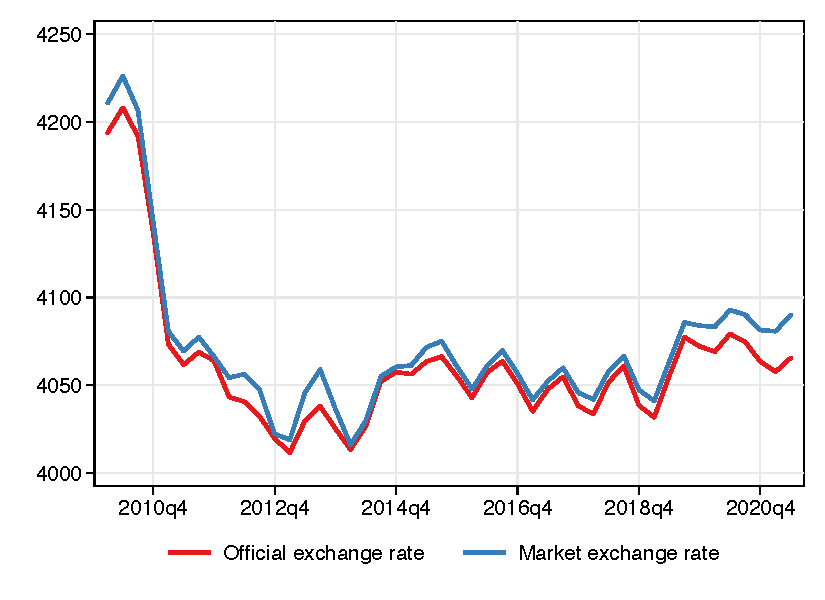
\includegraphics[width=0.7\linewidth]{../../empirical/Marcodata/Graphs/moving_exrate}
	\vspace{-1em}
	\begin{tablenotes}
		\footnotesize
		\item \textbf{Note:} This figure visualizes the moving average of the exchange rate \$1 to Khmer riels in the real price in the market and the official rate that set by the central bank during the period of 2010Q1--2021Q2. I plotted this figure based on the National Bank of Cambodia's dataset. 
	\end{tablenotes} 
	
\end{figure}

%-----------------------------------------------------------------------------------
In general, NBC has set the official exchange rate with a one percent difference compared to the market rate. The exchange rate Khmer riel against US dollar was set around 4,000 riels per \$1 unit. The exchange rate of Vietnam dong against Khmer riel and Thai baht against Khmer riel is associated with a bilateral exchange rate of US dollar against Vietnam dong and US dollar against Thai baht. 


Figure \ref{fig:1} reports the moving average of the change rate between Khmer riel and US dollar in the time period 2010Q1--2021Q2. The red line represents the exchange set by the central bank in terms of buying and selling in Khmer riel and US dollar. The blue line represents the real value of the exchange rate in the market. In fact, the Financial crisis of 2007--2008 affected the exchange rate in Cambodia in the short run. As a result, the value of Khmer riel raised 4,230 riels per \$1 unit in the first quarter of 2010. This means that the value of Khmer riel fell, leading to increased inflation and may negatively impact low-income households. Latter, from 2012Q1--2021Q2, the exchange rate between Khmer riel and US dollar has been stable with around 4,060 riels per \$1 unit. Even though the COVID-19 pandemic in 2020--2021 negatively impacted many economic sectors throughout the national, however, the exchange rate is seen not to increase much. This can reflect the effort of Cambodian monetary policy's economists acts well to control money supplies in the market. 

%-----------------------------------------------------------------------------------
\begin{figure}[H]
	\caption{The growth of the broad money and inflation during 2010Q1--2021Q2}
	\label{fig:2}
	\begin{subfigure}[b]{0.5\linewidth}
		\caption*{Panel A: Broad Money} \vspace{-.5em}
		\label{fig:2a}
		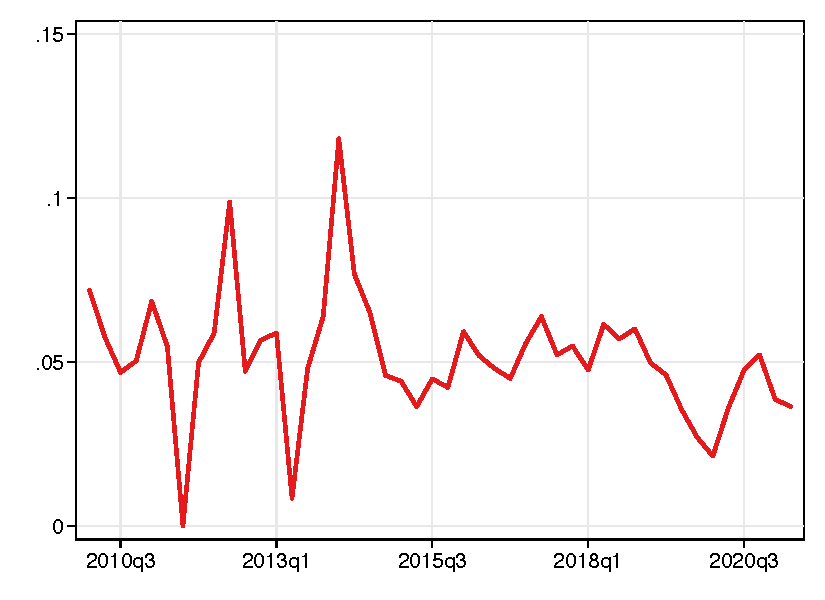
\includegraphics[width=1\linewidth]{../../empirical/Marcodata/Graphs/moving_m2} 
	\end{subfigure}%
	\hfil
	\begin{subfigure}[b]{0.5\linewidth}
		\caption*{Panel B: Inflation} \vspace{-.5em}
		\label{fig:2b}
		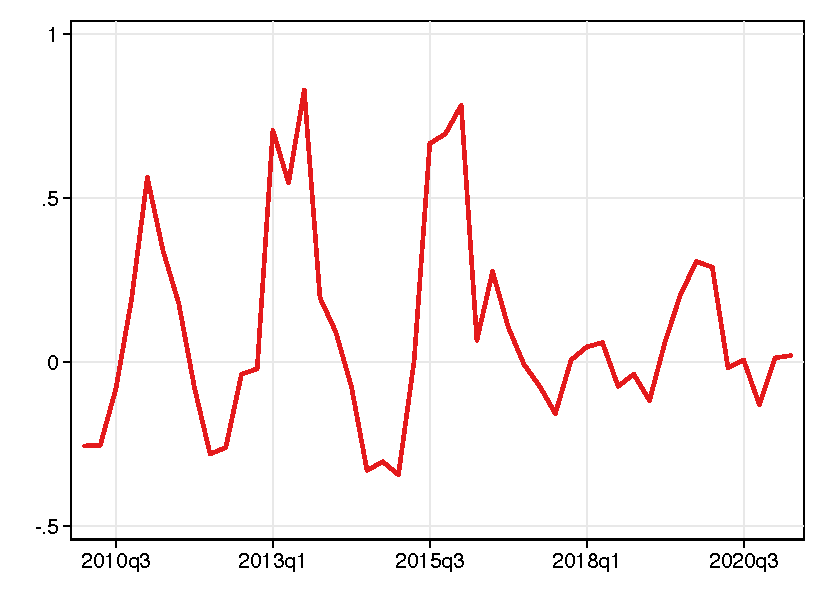
\includegraphics[width=1\linewidth]{../../empirical/Marcodata/Graphs/moving_inflation}
	\end{subfigure}
	\begin{tablenotes}
		\footnotesize
		\item \textbf{Note:} This two figures represent the moving average of the broad money and inflation between 2010Q1--2021Q2. Panel A reports the broad money and Panel B reports inflation rate growth. The $y$-axis reports the percentage change with multiply by 100 bias, the $x$-axis is the time period in quarters. The data uses to plot these figure come the National Bank of Cambodia and the National Institute of Statistics.  
	\end{tablenotes} 
	
\end{figure}

%-----------------------------------------------------------------------------------
In Cambodia, the local currency is estimated as just 10\% of the total board money. In \citet{Khou2013} documents that the circulation of Khmer riel has grown since the early 2000s, in particular, in the second half. Between 1989 and 2000, the number of riels in circulation varied slightly and was around \$100 million, while the economic growth rate exceeded 5\% on average. In contrast, it increased by about 20\% between 2001--2010. This allowed the volume of banknotes in circulation to pass from about \$100 million in the period of 1989--2000 to nearly \$800 million in 2010. At the same time, bank deposits in riels remain very low; it represents less than 5\% of total deposits. Figure \ref{fig:2} shows the moving average of broad money and inflation growth during 2010Q1--2021Q2. Panel A reports the broad money growth and Panel B is the inflation rate growth. The $y$-axis for both figure represents the percentage point change with multiply by 100. Both the broad money and inflation tend changed consistent similar between 2010Q--2014Q4. From a quarter to a quarter, the broad money supply changed around 5\%, while the inflation rate has a median about 30\%. 




Figure \ref{fig:3} reports the moving average of the overall inflation rate and its core consumer prices index (CPI) between 2010Q1--2021Q2. Overall, inflation has a median rate of about 3\% per year and 3\% per quarter. With the core food inflation, an average of around 2.4\% and core oil inflation usually tends below food CPI about 1\% on average in annual. 
%-----------------------------------------------------------------------------------
\begin{figure}[H]
	\centering
	\caption{The moving average of consumer prices index and the core CPI}
	\label{fig:3}
	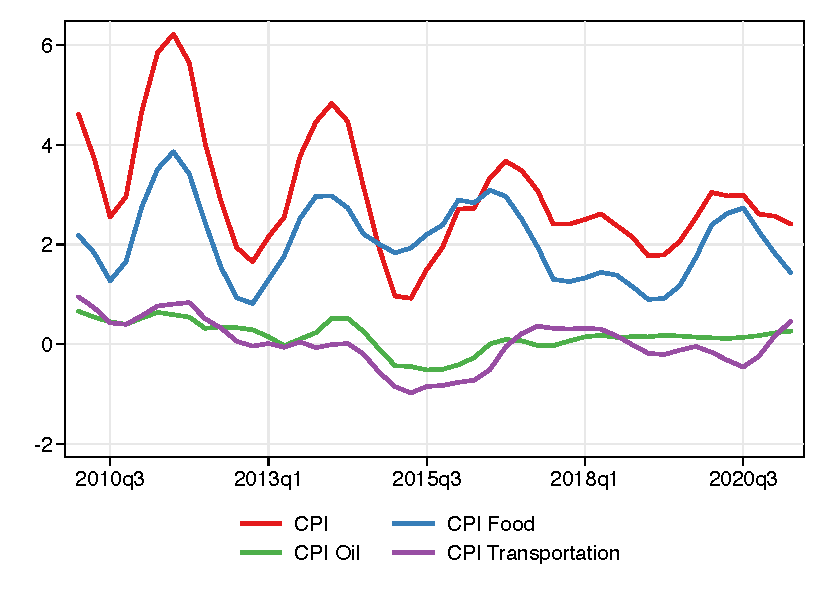
\includegraphics[width=.8\linewidth]{../../empirical/Marcodata/Graphs/moving_cpi} \vspace{-1em}
	
	\begin{tablenotes}
		\footnotesize
		\item \textbf{Note:} The figure reports the moving average of the CPI and core CPI in Cambodia between 2010Q1--2021Q2. The red line is the overall CPI, the blue line is the CPI for food, the green line reports the CPI oil and the purple is the CPI transportation. The $y$-axis is the rate of inflation and the $x$-axis is the time period in quarterly. I used the dataset from the National Institute of Statistics. 
	\end{tablenotes} 
	
\end{figure}


%-----------------------------------------------------------------------------------
It should be noted that the reserve requirement is main Cambodia's monetary policy to control the prudential and liquidity management. At the time of the pandemic, many economic activities were hard hit in demand and supply shocks. To facilitate a stable money supply in the market, the monetary policy committee deducted to reduce the reserve requirement for both local and foreign currency US dollar to 7\%.\footnote{The decision to continue with the rate of reserve requirement in 7\%, which was introduced since 2021. The summary result of the 56 Monetary Policy Committee Meeting was released on the official Facebook page of NBC on 23 August 2021. This settlement can be found via this link: \url{https://www.facebook.com/nationalbankofcambodiaofficial/photos/3897621040348119}} In common theoretical economy has shown that the monetary policy is the process which by the monetary administration of a country, like the central bank or currency board, controls the supply of money, usually targeting an inflation rate or interest rates to ensure price stability and general trust in the currency. Further goals of a monetary policy are usually to contribute to economic growth and stability, lower unemployment, and maintain predictable exchange rates with other currencies.

%-----------------------------------------------------------------------------------
\subsection{Household Monetary}
%-----------------------------------------------------------------------------------
In 2020, the total number of Cambodian households estimated about 3.6 million, which represents practically 15.9 million population living in Cambodia \cite{NIS2019}. The gross domestic product (GDP) per capita has increased from \$1,555 in 2018 to \$1,694 in 2019. Simultaneously, the total monthly disposable household income estimated to be \$567 in 2019/2020, which significantly increased by 16\% compared to 2017 and increased by 58\% compared to the year of 2014. 



The distribution of household income by income groups is presented in Figure \ref{fig:6}. Through the CSES data in 2017--2019/2020 by using sample weights of each three surveys, I estimate that the percentage of lower-income households who earned around under \$2,000--\$3,000 per annual raised about 1\% between 2014--2020. In which 34\% of total Cambodian households in 2014 increased to 35\% in 2020. At the same time, the percentage of higher-income households in the group of above \$12,000 to above \$15,000 significantly downed from 19\% in 2019 to 12\% in 2020. When the share of the median-income household (earned income between \$6,000--\$9,000 per year) has risen the proposition about 5\% during the last 7 years. 
%-----------------------------------------------------------------------------------
\begin{figure}[h]
	\caption{Household income group between 2014--2020}
	\label{fig:6}
	\begin{subfigure}[b]{0.33\linewidth}
		\caption*{Panel A: CSES 2014} \vspace{-.5em}
		\label{fig:3a}
		\includegraphics[width=1\linewidth]{../../empirical/CSES2014/Appendix/Graphs/groupinc} 
	\end{subfigure}%
	\hfil
	\begin{subfigure}[b]{0.33\linewidth}
		\caption*{Panel B: CSES 2017} \vspace{-.5em}
		\label{fig:3b}
		\includegraphics[width=1\linewidth]{../../empirical/CSES2017/Appendix/Graphs/groupinc} 
	\end{subfigure}
	\hfil
	\begin{subfigure}[b]{0.33\linewidth}
		\caption*{Panel C: CSES 2019} \vspace{-.5em}
		\label{fig:3c}
		\includegraphics[width=1\linewidth]{../../empirical/CSES2019/Appendix/Graphs/groupinc} 
	\end{subfigure}
	\begin{tablenotes}
		\footnotesize
		\item \textbf{Note:} The figure presents the household income group by using income data from the 2014--2019/2020 CSES . Panel A reports the household income group in 2014, Panel B is the household income group in 2017, and Panel C is the income group in 2019--2020. All three graphs used sample weights, and removed the lower- and higher-income household 1\%.  
	\end{tablenotes} 
\end{figure}

%-----------------------------------------------------------------------------------

Due to a lack of financial sources for household investment and consumption, many households took loans from banks, microfinance institutions and moneylenders. As the socioeconomic survey, Cambodian households taking loans for different propose, in particular, some taking loans for production and economic activities, some for household consumption both in durable goods and food goods, some households are taking credits for repayment other interest banks, preparing the party, and other purposes. The purpose of households taking a loan is reported in Figure \ref{fig:8}. The percentage of households taking loans for business purposes has declined over time, which is nearly 39\% in 2014 has decreased to 30\% in 2019/2020. At the time, we have seen that loans for consumption raised 3\%, from 58\% in 2014 to 61\% in 2019/2020. Households taking credit for repayment other loans raise their proposition about 3\% from 2014 to 2020. In terms of liabilities, each household has a different interest rate payment, as shown in section \ref{sec:appirate} in the Online Appendix. 

%-----------------------------------------------------------------------------------
\begin{figure}[h]
	\caption{ The purposes for household loans over 2014--2020}
	\label{fig:8}
	\begin{subfigure}[b]{0.33\linewidth}
		\caption*{Panel A: CSES 2014} \vspace{-.5em}
		\label{fig:3a}
		\includegraphics[width=1\linewidth]{../../empirical/CSES2014/Appendix/Graphs/loan_reason} 
	\end{subfigure}%
	\hfil
	\begin{subfigure}[b]{0.33\linewidth}
		\caption*{Panel B: CSES 2017} \vspace{-.5em}
		\label{fig:3b}
		\includegraphics[width=1\linewidth]{../../empirical/CSES2017/Appendix/Graphs/loan_reason} 
	\end{subfigure}
	\hfil
	\begin{subfigure}[b]{0.33\linewidth}
		\caption*{Panel C: CSES 2019} \vspace{-.5em}
		\label{fig:3c}
		\includegraphics[width=1\linewidth]{../../empirical/CSES2019/Appendix/Graphs/loan_reason} 
	\end{subfigure}
	\begin{tablenotes}
		\footnotesize
		\item \textbf{Note:} The figure presents the objective of household loans  by using liabilities data from the 2014--2019/2020 CSES. Panel A reports the purpose of household loan in 2014, Panel B is the household loan purpose in 2017, and Panel C is the credit objective in 2019--2020. All three graphs used sample weights, and removed the lower- and higher-liability household 1\%.  
	\end{tablenotes} 
	
\end{figure}

%------------------------------------------------------------------
\section{Data}\label{sec:data}

This section describes the data source and samples used to analyze the impact of monetary policy shock on economic variables and monetary policy on the household economy.   

%-----------------------------------------------------------------
\subsection{Macroeconomic Variables}	

I used macroeconomic variables such as inflation, the exchange rate, the interest rate, unemployment, broad money supply in the market, and real GDP growth as the main interest variables applied in analyzing the effect of monetary policy on economic structure. The primary sources of these variables come from the NBC, the National Institute of Statistics of Cambodia (NIS) and the International Labor Organization (ILO). NBC databases are available online on their official website.\footnote{We can download a more recent dataset on the financial sector at the National Bank of Cambodia’s website: \url{https://www.nbc.org.kh/english/economic_research/monetary_and_financial_statistics_data.php}.} Most of the NBC data set is focused on monetary, banking, financing, microfinance, the balance of payment, interest rates, and exchange rates. 

I collected inflation and industrial output growth (GDP) data from the NIS through the National Account Statistics Table (SNA).\footnote{The National Account Statistics of Cambodia can be found here: \url{https://www.nis.gov.kh/index.php/km/21-na/41-national-accounts}.} The SNA of Cambodia was first built in 1993 and the estimation was up to date every year. With the technical support from the Asian Development Bank, the NIS authorities can produce the SNA through three main approaches like production, expenditure and income approach. It should be noted that GDP data comes from the sum of three broad economic sectors like agriculture, industry and services. At the same time, GDP is estimated on both production and expenditure approach and at current prices as well as at constant 2000 prices. 

In this paper, I selected a time series of macroeconomic variables from the period of 2010Q1--2021Q2, equivalent to 44 observations. In fact, I do not have real output growth data in the quarter. To get output in quarters, I assume all quarter periods in a year have the same proposition throughout the year. Thus, I divided output growth per year with 4 to take data in quarters. The employment rate is the same, I divided it by 4 to get the rate in quarters. 

Table \ref{app:tabm1} in the Online Appendix reports summary statistics of main macroeconomic variables that are used for empirical analysis. Surprisingly, developing economies like Cambodia have experienced one of the poorest countries in the region with a shallow employment rate, barely 0.31 percent in 2020. However, some say that the estimation warns that the number does not tell the entire story. Still, it probably is a problem with the unemployment rate definition. Based on the ILO, they account for all informal sectors, who have to work a few hours in a week both for received paid and unpaid, in the meantime, they are looking for another job and another source of income.\footnote{This is a statement said by former head economist Sera Elder of the ILO’s Asia and Pacific in 2018 at the Phnom Penh Post: \url{https://www.phnompenhpost.com/national/cambodias-low-rate-unemployment-doesnt-tell-whole-story-report-finds}.}


%-----------------------------------------------------------------------------------

\subsection{Household Survey Data}\label{sec:data2}	
%-----------------------------------------------------------------------------------

To be able to analyze the heterogeneous effects of monetary policy shocks on households, I need detailed microdata on consumption expenditure, income, assets and liabilities at a regular frequency for a sample spanning the last seven years from Cambodia during 2014--2020 through the Cambodia Socio-Economic Survey (CSES) of the NIS. 

The CSES is a large sample size household survey in Cambodia conducted in 1993 by the Ministry of Planning and the regulatory conduct up to date every two years with the new sample size and new random household respondents. The CSES is the most significant survey on household living conditions. It provides high-quality, detailed information on household characteristics variables, consumption, income sources, tangible assets, various debt components, economic activities and other indicators that are very useful for socioeconomics study. The CSES is a popular source for economists who study Cambodia.\footnote{\citet{Seng2018} used the CSES 2014 to study the effects of microcredit on household poverty in terms of food consumption and \citet{Phoumin2019} applied the CSES 2015 to investigate the impacts of energy consumption on the health, education and earning opportunities of the family. Interestingly, \citet{Saing2019} used a large sample size of the CSES between 2004--2010 to analyze his empirical study of the long term effect of US bombing during the 1969--1973 period on education, earnings, health, fertility and marriage in Cambodia.} 

Indeed, household surveys have been used by several studies on the impact of monetary policy on income inequality (e.g., \citet{Coibion2017, Jappelli2014} for the U.S.; \citet{Mumtaz2017} for the U.K.; \citet{Inui2017} for Japan; and \citet{Casiraghi2018} for Italy). To the best of my knowledge, I compiled a repeated cross-section based on the last 7 waves, spanning the period from 2014 to 2020. Each wave contains different observations. For instance, the CSES 2014 has observed around 12,000 households, the CSES 2017 has a small observation with around 3,800 households and the CSES 2019/2020 has approximately 10,000 observations. Although the CSES has different sample sizes over time, it still covers a representative sample of the Cambodian resident population. Data is collected through personal interviews. Questions concerning the whole household are addressed to the household head or the person most knowledgeable about the family’s finances. The unit of observation is the family, which is defined as including all persons residing in the same dwelling who are related by blood, marriage, or adoption as well as individuals described as partners or other common-law relationships are also treated as family. 

According to the CSES dataset, I generated 10 main variables for the purpose of analysis of household income inequality. Specifically, net household income ($Y_{i}-T_{i}$), household consumption ($C_{i}$), maturing assets ($A_{i}$), maturing liabilities ($L_{i}$), unhedged interest rate exposure ($URE_{i}$), nominal household assets, nominal household liabilities, net nominal position ($NNP_{i}$), gross income ($Y_{i}$), and average propensity to consume ($APC_{i}$). For more information about our methodology to remove outliers and how to make quality data reliable and valid, see Online Appendix \ref{app:tabdata}. 

Ideally, I would like to observe how a household or individual income and consumption expenditure evolve over time. Unfortunately, I cannot do that because the CSES is a repeated cross-section with no such panel dimension. It is not possible to analyze and estimate the marginal propensity of consume (MPC) of each household. However, in the previous literature, such as \citet{Browning1985, Deaton1985} and \citet{Gardes2005} have constructed a pseudo-panel through time-series and cross-section surveys in a way making it possible to analyze the included data as if they originated in a genuine panel data set. It is a standard method consisting of cohorts of individuals in the survey, for instance by age, gender, education, region, income and consumption, and use conventional methods for panel data to analyze the pseudo-panel.\footnote{Each method has its own limitation, pseudo-panels can significantly reduce the number of observations. For example, if I build 16 cohorts within 3 years of observed household information in my data set, I will take only 48 observations throughout the CESE 2014--2019.} Nevertheless, I do not apply the pseudo-panel to this paper due to a small time-series data record.  

No matter how complete, survey data on household economics and demographic characteristics lack explicit measures of all possible factors that might bias the estimates. The CSES 2014 differs from the other, especially for self-employment income data. This is the leading cause of a significant increase in average disposable income compared to the CSES 2017 and 2019/2020. The main reason behind this is that they conducted more interviews with many household business owners. If I dropped household business income in 2014, the median household income across the country in this year is reasonable given the trend growth like other (not much high) in 2017 and 2019, see in Table \ref{tab:g1}, but that is not the case in this paper because it will lose over 3,800 observations and turn the problem into other variables such as household wages and farm incomes. 

Simultaneously, the total household income is the same, many households do not report their income sources because it is difficult to estimate and get data on families working in agriculture, their own account worker and unpaid family worker.\footnote{This is a technical issue that has been mentioned in every CSES report \cite{NIS2019}.} There is a thing that is very challenging for me, many families have zero and minimal income reported whereas high consumption expenditure that negatively impacts welfare. In particular, many households reported negative annual income of more than 10--50\% even though I account that taking loans as a part of family consumption. 

Tables \ref{app:tab1}--\ref{app:tab3} in the Online Appendix present summary statistics for the main variables used in my estimation. All statistics are computed using survey weights. In general, the CSES recorded the amount of value in Khmer riels. Therefore, I converted its value to US dollar in terms of the annual real exchange rate of the baseline year.\footnote{The baseline year of these three surveys is 2014, 2017, and 2019.} To do so, it will be easy to compare with other developing economies that have the same economic structure and condition, but I do not do the comparison in this paper. From 2014--2020, the median household wages across the nation have increased significantly with the growth rate of 28.71\%, which is \$1,978 in 2014, \$2,781 in 2017, and \$3,249 in 2020. The annual average household agricultural income has trended unstable during the last 7 years. It recorded \$1,242 in 2014, \$886 in 2017 and \$1,323 in 2020. Furthermore, Cambodia’s households experienced increasing consumption expenditure between 2014 to 2020. The average change is 16.90\% in the period due to the change of income, inflation and other economic variables that are associated with consumption. A thing that consists of making a change of total consumption is food consumption. As the survey showed, each household reported increased food consumption. Additionally, for more detail about variables and descriptive statistics, see Online Appendix \ref{app:tabdata}.

%-----------------------------------------------------------------------------------
\section{A Model of Monetary Policy Transmission Channel}\label{sec:r1}
%-----------------------------------------------------------------------------------
%-----------------------------------------------------------------------------------

\subsection{Monetary Policy Transmission}
%-----------------------------------------------------------------------------------
	Describing and summarizing data, making macroeconomic forecasts, quantifying what we know or do not know about the real structure of the macroeconomics, and advising macroeconomic policy makers are the main things macroeconometricians have been doing for a long time. By the 1970s, the four tasks were performed using a variety of techniques. These ranged from large models with hundreds of equations to single-equation models that focused on interaction of a few variables to simple univariate time series models involving only a single variable.  


	A decade ago, these approaches appeared especially trustworthy. In fact, since the seminal work of \citet{Sims1980} provides a new maroeocometric framework on structural vector autoregressions (SVAR) have evolved into one of the most widely used models in empirical research using time series data. It is a univariate autoregression (a single equation or single variable linear model) in which the current value of a variable is explained by its own lagged values. 

	A VAR is an $n$-equation, $n$-variable linear model in which each variable is in turn explained by its own lagged values, plus current and past values of the remaining $n - 1$ variables. This simple framework provides a systematic way to capture rich dynamics in multiple time series, and the statistical toolkit that came with VARs was easy to use and to interpret.\footnote{Standard practice in VAR analysis is to report results from Granger causality tests, impulse responses and forest error variance decompositions. These statistics are computed automatically or nearly so by many econometrics applications such as RATS, Eviews, TSP, Stata and others.} Over time, many new ideas have been coming and explored, sometimes uncritically applied or misunderstood by practitioners, the unquestioned, and later refined or replaced by alternative methods. The development of new methods of identification, estimation, and inference for structural VAR models continues at a rapid pace even today. 	
	
	Let consider $Y_{t}$ be the $n\times 1$ vector of time series observable variables. My reference reduced form model is given by the VAR system with constant parameters:
	
	\begin{equation}\label{eq1}
	Y_{t} = A_{1}Y_{t-1} + A_{2}Y_{t-2} +  \cdots + A_{l}Y_{t-l} + \Psi D_{t} + u_{t}, \:\:\:\:\:\: t = 1, \cdots, T  
	\end{equation}

	\noindent where  $u_{t}$ is a $n$-dimensional one-step ahead prediction error or white noise with positive definite time-invariant covariance matrix $\sum_{u} = E(u_{t}u'_{t})$. $A_{j}, j = 1,\cdots,l$ are coefficient matrices of size $n\times n$, $l$ is the VAR lag order and $D_{t}$ is an $m$-dimensional vector containing deterministic components that can be constant, trend and dummies. $\Psi$ is the $n\times m$ matrix of associated coefficients and $T$ is the sample length.        
	
	The disagreement starts when discussing how to decompose the prediction error $u_{t}$ into economically meaningful or fundamental innovations. This is necessary because one is typically interested in examining the impulse responses to such fundamental innovations, given the estimated VAR. In particular, much of the literature is interested in examining the impulse responses to a monetary policy innovation.
	
	I compact the VAR system equation (\ref{eq1}) in the expression
	
	\begin{equation}\label{eq2}
		Y_{t} = \prod W_{t} + u_{t},  \:\:\:\:\:\: t = 1, \cdots, T  
	\end{equation}
	
	\noindent where $W_{t} = (Y'_{t-1}, \cdots, Y'_{t-l}, D'_{t})$ and $\prod = (A_{1}, A_{2}, \cdots, A_{l}, \Psi)$. The matrix $\prod$ is $n \times f, f = dim(W_{t}) = nl+m$ and the VAR reduced from parameters are collected in the $p$-dimensional vector $\theta = (\pi', \sigma'_{+})'$, where $\pi = \mathrm{vec}(\prod)$ and $\sigma_{+} = \mathrm{vech}(\sum), p = nf+\frac{1}{2}n(n+1). 
	
	Suppose that there are a total of $n$ fundational innovation, which are mutually indenpendent and normailzed to be of variance 1, thus, the SVAR is interested in this paper is defined by 
	
	\begin{equation}\label{eq3}
		u_{t} = Bv_{t}, \:\:\:\:\: E(v_{t}v'_{t}) = I_{n}, \:\:\:\:\: \sum_{u} = BB'
	\end{equation}

	\noindent where $B$ is a non-singular $n \times n$ matrix of structural parameters and $v_{t}$ is a $n$-dimensional independent and identically distributed (i.i.d.) vector of structural shocks with covariance matrix normalized to $I_{n}$. As we known, the system (\ref{eq2})--(\ref{eq3}) is unidentified without any restriction on the elements of the $B$ matrix. The standard way to achieve identification is to include a set of linear restriction on $B$ that I can write in explicit form
	\begin{equation}\label{eq4}
		\mathrm{vec}(B) = G_{B} \gamma  + g_{B}
	\end{equation}

	I propose to go all the way by only concentrating on finding the innnovation corresponding to the monetary policy shock. In equation (\ref{eq4}), $G_{B}$ denotes a $n^2 \times a_{B}$ selection matrix, $\gamma$ is $a_{B} \times 1$ and contains the free elements of $B$, and $g_{B}$ is a $n^2 \times 1$ vector. This amounts to identify a signle colunm $a \in \mathbb{R}^{m}$ of the matrix $B$ in equation (\ref{eq3}). The information required to specify the matrix $G_{B}$ and the vector $g_{B}$ usually comes from the economic theory or from structural and institutional knowledge related to the problem under study. The condition $a_{B} = dim(\gamma)\leq n(n+1)/2$ is necessary for identification. The necessary and sufficient condition for identification is that the $n(n+1)/2 \times a_{B}$ matrix
	\begin{equation}\label{eq5}
		2D_{n}^{+}(B \bigotimes I_{n})G_{B}
	\end{equation}

	\noindent has full column rank evaluated at $B_{0}$ where $B_{0}$ denotes the counterpart of $B$ that fulfills the restriction $\mathrm{vec}(B_{0}) = G_{B} \gamma_{0} + g_{B}$, and $\gamma_{0}$ is the true value of $\gamma$. 
	
	To avoid confusion, throughout the paper I call reduced from parameters the elements in the vector $\theta$, and structural parameters the elements of the vector $\gamma$ and possibly, the variances of the structural shocks $e_{t}$ when these are not normalized to one. If the rank condition in equation (\ref{eq5}) holds, the orthogonalized impulse reponse function (IRFs) are taken from the matrices $\Gamma_{h}$ = \begin{bmatrix}
	\Psi_{km,h}\end{bmatrix} = \Phi \breve{B} = (J'\mathring{A}^{h}J) $\breve{B}, h =0,1,2 \cdots$, where 

	\begin{equation}\label{eq6}
	\mathring{A} = \begin{pmatrix}
			A_{1} & A_{l}   \\
			I_{n(l-1)},& 0_{n(l-1)\times n} \\
		\end{pmatrix}
	\end{equation}

	\noindent is the VAR compansion matrix, $J =(I_{n}, 0, \cdots, 0)$ and \breve{C} denotes a specification of $B$ such that matrix in equation (\ref{eq5}) has full column rank. The coeffcient $\Psi_{km,h}$ captures the reponse of variable $k$ to a one-unit impulse in variable $m,h$ periods before.\footnote{The identification of $C$ can also be achieved by complementing the symmetry restrictions $\sum=BB'$ with a proper set of constraints on the matrix 
	\begin{equation*}
	\Gamma_{\infty} = (I_{n}-A_{1} \cdots - A_{l})^{-1}B = \sum_{h=0}^{\infty}\Phi_{h}B = J'(I_{nl}-\mathring{A})^{-1}JB 
	\end{equation*}
	\noindent which measures the long-run impact of the structural shocks on the variables \cite{Blanchard1989}. Constraints
	on $\sum_{infty}$ can be used in place of, or in conjunction with, the ‘short run’ restrictions in equation \ref{eq4}).
}

	In this paper, the specification of the SVAR model is based on a standard moneteary VAR model that apperar in \citet{ Bacchiocchi2015, Christiano2005, Christiano1999, Stock2001}; and \citet{Uhlig2005}
	
	To make it short, the SVAR model of this study can rewritten as follows: 
		\begin{equation}\label{eq7}
		 	Y_{t} =\begin{bmatrix} 
			\pi_{t} \\
			y_{t} \\
			i_{t}\\
			u_{t} \\
			log(E_{t}) \\
			log(M2_{t})
		\end{bmatrix}, \:\:\:\:\:\: t = 1, \cdots, T
	\end{equation}
	
	As shown in the equation (\ref{eq7}), this is the monetary aggregate composed use in my paper. The $\pi$ is inflation componse to time series $t$, $y$ is output, $i$ denotes as the interest rate, $u$ is the umemployment rate, $E$ and $M2$ are the exchange rate and broad momey with logarithm.  
%------------------------------------------------------------------
\subsection{Results} 
In this section, I provide detailed discussion on my main results of the monetary policy shocks through the SVAR model in equation (\ref{eq1}). First, I present the result of Granger causality tests and second, I present the impulse response of monetary policy to macroeconomic variables.  

%-----------------------------------------------------------------------------------
\subsubsection{The Granger Causality Tests}
%-----------------------------------------------------------------------------------

Table \ref{tab:gvar} summarizes the Granger-causality results for the six-variable VAR. It shows the $p$-values associated with the chi-squared statistic for testing whether the relevant sets of coefficients are zero. For example, if inflation does not help predict broad money, then the coefficient on the lags of inflation will all be zero in the reduced-form broad money supply equation. Inflation does not helps predict the broad money ($M2$), the unemployment rate, the exchange rate and the interest rate levels of statistical significance. Nevertheless, inflation helps predict output at the 10\% significance level with the $p$-value 0.076 or 7.6\%. My Granger tests show the $M2$ significantly impacts output, inflation and exchange rates at 1\% and 5\% of statistical significance (the $p$-value is 0.004, 0.017, and 0.036, respectively). In addition, the results reflect that the use of exchange rates as an instrument policy to control money supply in the market has a true consensus effect on other macroeconomic variables. As we see in Table \ref{tab:gvar}, the exchange rate has Granger-cause broad money and output statistically significant at a 1\% and 5\% level with $p$-value is 0.001 or 1\% and 0.097 or 9.7\%. Surprisingly, the unemployment rate has a consequence to many economic variables like inflation at a 1\% of statisitical significance, to $M2$ (4.9\%), the interest rate (4\%), and exchange rates at $p$-value 0.019 or 1.9\%. 

\begin{table}[h!]
	\centering
	\caption{Granger Causality Tests for VAR Model}
	\label{tab:gvar}
	\resizebox{\textwidth}{!}{%
		\begin{tabular}{@{}lcccccc@{}}
			\hline \hline
			Regressor & Inflation & M2    & Output & Unemployment & Exchange rate & Interest rate \\ \hline
			Inflation          &    ---       & 0.000 & 0.076  & 0.510        & 0.162         & 0.493         \\
			M2                 & 0.004     &    ---   & 0.017  & 0.555        & 0.000         & 0.036         \\
			Output             & 0.045     & 0.078 &     ---   & 0.153        & 0.000         & 0.000         \\
			Unemployment       & 0.010     & 0.049 & 0.405  &      ---        & 0.019         & 0.040         \\
			Exchange rate      & 0.131     & 0.001 & 0.097  & 0.973        &        ---       & 0.158         \\
			Interest rate      & 0.007     & 0.000 & 0.014  & 0.000        & 0.000        &      ---         \\ \hline \hline
		\end{tabular}%
	}
	\begin{tablenotes}
		\small
		\item \textbf{Note:} All entries are chi-square test statistics at dregress of freedom with an indicate significant at 1\%, 5\% and 10\% levels, parentheses are $P$-values. The row labeled \textit{Regressor} do not enter the reduced form equation for column variable labeled \textit{Dependent Variable}. The results were computed from a VAR with four lags and a constant term over the 2010Q1--2021:Q2 sample period. 
	\end{tablenotes} 
	
\end{table}    
%-----------------------------------------------------------------------------------
\subsubsection{The Effects of Monetary Policy Shocks}
Impulse response traces out the response of the current and future trend values of each variable interest to a one-unit increase in the current value of one of the SVAR errors. I assume that this error returns to zero in subsequent periods and that all other errors are equal to zero. Of course, the SVAR methods outlined here have some limitations. One is that computing standard errors for impulse responses probably give misleading results if some variables are highly persistent. To respond in terms of errors, I decided to use output and the exchange rate with logarithm.  

%-----------------------------------------------------------------------------------
\begin{figure}[H]
	\centering
	\caption{Inpulse response in the exchange rate--inflation--output--unemployment in SVAR}
	\label{fig:4}
	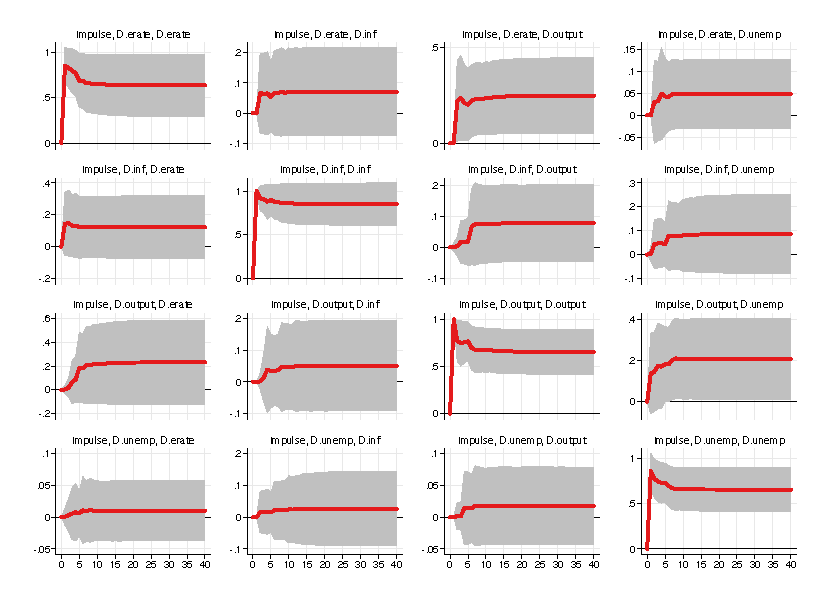
\includegraphics[width=1\linewidth]{../../empirical/Marcodata/Graphs/var_svar1}
	
	\begin{tablenotes}
		\footnotesize
		\item \textbf{Note:} This figure reports the impulse response of monetary policy shocks through the SVAR model on inflation, the interest rate, the exchange rate and output over the horizon 1 to 42 quarters (a constant duration over the sample period 2010Q1–2021Q2) with four lags. All $y$-axis shows the percentage deviation from the pre-shock levels. The red line is the point estimates and the grey area shows 95\% bootstrapped confidence intervals for each impulse response. All $x$-axis is the time period in quarters. The first row is the exchange rate shock, the second row is inflation shock, the third row is output shock, and the last row is the unemployment shock. 
		
	\end{tablenotes} 
\end{figure}
%-----------------------------------------------------------------------------------
Figure \ref{fig:4} reports the impulse responses of the endogenous variables to the standard deviation shock in the exchange rate, inflation, output and unemployment. The first row shows the effect of an unexpected percentage point increase in the exchange rate on all four endogenous variables, as it works through the SVAR system with the coefficients estimated from actual data. The second row reports the effect of an unexpected percentage point in inflation on the exchange rate, inflation, output and unemployment, with the coefficients estimated from actual data as the same as the first row.  The third and fourth rows provide information on the effectiveness of output growth and the unemployment rate on all four interest variables. The solid red lines are the point estimates and the shaded gray areas are 95\%, confidence bands. 


The exchange rate is a significant monetary policy instrument in Cambodia that the central bank plays around with its innovation to control the money supply and inflation in the country as a whole. However, a restrictive monetary exchange rate of US dollars and Cambodian riels leads to a robust and immediate increase in the component of inflation, output and unemployment rate. However, the trend is no longer persistently increasing, it seems consistent in the long run. In terms of magnitudes, the exchange rate policy shock responds to increasing inflation and the unemployment rate by 0.06\% and 0.05\%. At the same time, it also causes an increase in nominal output by around 0.2\% points, but the growth no longer exists. It seems to decrease about 0.03\% in the 5 quarters and then start to recover with consistent trends in the long run by about 0.25\%. 

As shown in the second row, the exchange rate, output, and unemployment have a different correspondence to inflation shock. The exchange rate statistically rose by 0.15\% from the 1 quarter, and the trend tightening fell in the two five quarters and tightening was consistent in the long run. The impulse response of real GDP growth to inflation has been low, increased 0.07\% point from zero to seven quarters and the trend seemed stable. Moreover, the unemployment rate has a low response to inflation, only 0.08\% in terms of magnitude. 


Financial variables that impulse response to unemployment are deficient, as seen in the fourth row. In particular, the exchange rate has a significant positive impact on the unemployment shock at 0.01\% in the short run, specifically, in 5 quarters. Output has been affected 0.02\% at 7 quarters, and the trend continues to be constant. Interestingly, even though sometimes inflation is unstable, the correction between inflation and the unemployment rate does not impact each other. It affects around 0.03 and 0.04\% points in 5--10 quarters and tends to be constant. 

Figure {\ref{fig:varsvar2} presents the SVAR impulse response of inflation, the interest rate, broad money, and output to its shock. The impulse response of the interest rate, $M2$ and output have shown in the first row. As we can see, all three endogenous variables positively impact on inflation shock. Especially, output has been a significant response to inflation over time, with the magnitude around zero in the baseline period to 0.1\% in 40 quarters. The interest rate positively impacts inflation shock around 0.2 in zero one quarter and down up around 0.02 or 0.03 in 5 quarters. However, it started to recover with around 2.3\% in 10 quarters and was consistent with reallocation friction in the economy. As a result, the responses are statistically and economically significant. The third column in the first row reports the impulse response of broad money to inflation shock. In terms of magnitudes, inflation policy shock increased broad money in the market around 0.07\% during the zero to ten quarters. The $M2$ response trunks out to be particularly pronounced, consistent with the long run. 
	%-----------------------------------------------------------------------------------
\begin{figure}[H]
	\centering
	\caption{Inpulse response in inflation--the interest rate--broad money--output in SVAR}
	\label{fig:varsvar2}
	\vspace{-1em}
	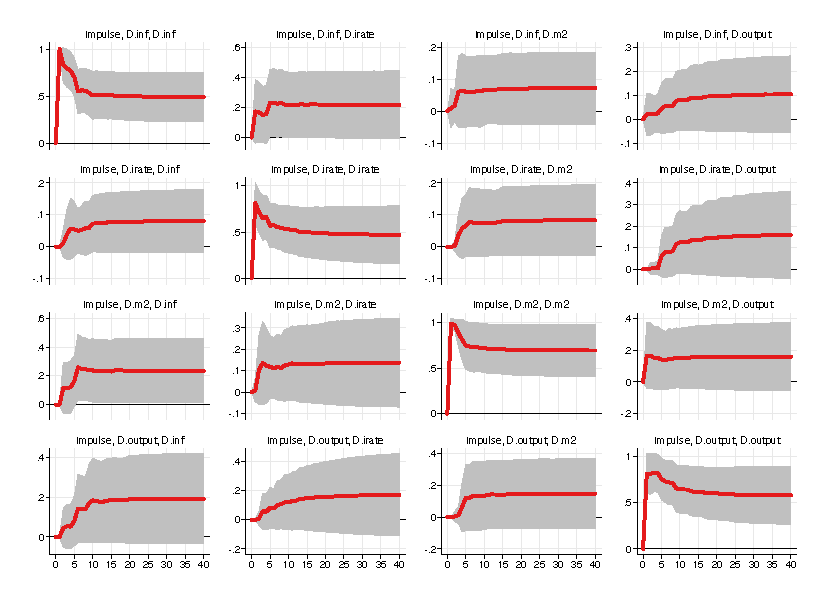
\includegraphics[width=1\linewidth]{../../empirical/Marcodata/Graphs/var_svar2}
	\vspace{-2.5em}
	\begin{tablenotes}
		\footnotesize
		\item \textbf{Note:} This figure reports the impulse response of monetary policy shocks through the SVAR model on inflation, the interest rate, broad money and output over the horizon 1 to 42 quarters (a constant duration over the sample period 2010Q1–2021Q2) with four lags. All $y$-axis shows the percentage deviation from the pre-shock levels. The red line is the point estimates and the grey area shows 95\% bootstrapped confidence intervals for each impulse response. All $x$-axis is the time period in quarters. The first row is the monetary policy shock through inflation shock, the second row is the interest rate shock, the third row is broad money shock, and the last row is output shock. 
		
	\end{tablenotes} 
\end{figure}
%-----------------------------------------------------------------------------------

	The second row shows the result of inflation, broad money and output response to the interest rate shock. The interest rate shock led to increasing inflation or consumer prices and money supply by around 0.08\%, and slightly raised output about 0.15\% point. On the other hand, the board money shock is through somewhat financial economic variables that are present in the third row. The interest rate, inflation and output response are complementary positive to the $M2$ shock. In terms of magnitudes, the $M2$ shock increased inflation value by 0.23\%, 0.13\% for interest rates, and around 0.18\% for output. 

	At the same time, I also analyze the variance percentage the error made in the forecasting a variable due to a specific shock. Tables \ref{app:tabv1}--\ref{app:tabv2} in the Online Appendix present the forecast error decomposition of main monetary shock with its monetary aggregate at a given horizon.\footnote{The forecast error decomposition is like a partial $R^2$ for the forecast, by forecast horizon.} 
%------------------------------------------------------------------
\section{Household Monetary Transmission Channels}\label{sec:r2}
In this section, I describe the theoretical model of aggregate consumption and the redistribution channel of monetary policy based on \citet{Auclert2019}, the empirical result by the household survey, measurement error through redistribution covariances and robustness checks.   

\subsection{Household Heterogeneity and Aggregate Consumption}
\subsubsection{Household Environment}
Consider a household with separable preference over nondurable consumption $c_{t}$ and hour of work $n_{t}$. I assume no aggregate uncertainty for simplicity: the same insights obtained when markets compete, except concerning idiosyncratic shock to their income and spending needs. The household endowed with a stream of real unearned income $y_{t}$. The family has perfect foresight over the general level of price $P_{t}$ and the path of the nominal wages $W_{t}$, and holds long-term nominal and real contracts. The time horizon is finite or infinite with discrete period $t= 0, 1, 2, \ldots$ and the agent solves the following utility maximization function:  

%-----------------------------------------------------------------------------------
\begin{equation*}
	\max \quad \mathbb{E} \left[\sum_{t=0}^{\infty}\beta^{t}\begin{Bmatrix}u (c_{t}) - v(n_{t})\end{Bmatrix}\right]
\end{equation*}
%-----------------------------------------------------------------------------------
%-----------------------------------------------------------------------------------
\begin{equation}\begin{split}\label{e1}
		\text{s.t.} \quad \quad P_{t}c_{t} = P_{t}y_{t} + W_{t}n_{t} + (_{t-1}B_{t}) + \sum_{s \geqslant 1}(_{t}Q_{t+s})(_{t-1}B_{t+s} - _{t}B_{t+s}) + P_{t}(_{t-1}b_{t}) \\
		+ \sum_{s \geqslant 1}(_{t}q_{t+s}) P_{t+s} (_{t-1}b_{t+s} - _{t}b_{t+s})
\end{split}\end{equation}
%-----------------------------------------------------------------------------------
The follow budget constraint in equation (\ref{e1}) views the househols' consumption in every period $t$, as having a portfolio of zero coupon bonds inherited from period $t-1$ and a portfolio of bonds to carry into the next period.\footnote{Of course, just decide to roll over their position from the previous period. This corresponds to the costless trade that sets $_{t-1}b_{t+s} $$= $$_{t}b_{t+s}$ and $_{t}B_{t+s}$$=$$ _{t-1}B_{t+s}$ for all $s$} $_tQ_{t+s}$ denotes the time $t$ price of a nominal zero coupon bond paying at time $t+s$ and $_{t}q_{t+s}$ is the price of a real zero coupon bond. $_{t}B_{t+s}$ denotes the nominal quantities purchased and $_{t}b_{t+s}$ is the real quantities purchased by households in each period, respectively. To keep the problem well-defined, I assume that the prices of nominal and real bonds prevent arbitrage profits. This implied a Fisher equation for the nominal term structure: 
%-----------------------------------------------------------------------------------
\begin{equation*}
	_{t}Q_{t+s} = (_{t}q_{t+s}) \frac{P_{t}}{P_{t+s}} \quad \quad \quad \forall t,s
\end{equation*}
%-----------------------------------------------------------------------------------
As I focus on the period $t=0$, financial nominal and real assets can be rewrites as: $_{-1}B_{t\geq 0}$ and $_{-1}b_{t\geq 0}$. Letter, I represent stocks, inflation and price-level adjusted mortgages. I write the real wage at $t$ as $w_{t} \equiv \frac{W_{t}}{P_{t}}$, the initial real term structure as $q_{t} \equiv {_{0}q_{t}}$, the initial nominal term structure as $Q_{t} \equiv {_{0}Q_{t}}$, and impose the present-value normalization $q_{0} = Q_{0} =1$.

Using either a terminal condition, the flow budget constraints consolidate into an intertemporal budget constraint: 
%-----------------------------------------------------------------------------------
\begin{equation}\label{e2}
	\sum_{s \geqslant 0}q_{t}c_{t} = \underbrace{\sum_{s \geqslant 0}q_{t}(y_{t} + w_{t}n_{t})}_{\omega^H} + \underbrace{\sum_{s \geqslant 0}q_{t}\left ( (_{1}b_{t}) + \left(\frac{_{1}B_{t}}{P_{t}}\right)\right )}_{\omega^F} \equiv \omega 
\end{equation}
%-----------------------------------------------------------------------------------
where consumption must equal be to wealth $\omega$, $\omega^{H}$  is the sum of household wealth that equivalent to the present value of all future income, and $\omega^{F}$ is the financial wealth. 





Since $_{-1}B_{t}$ and $_{-1}b_{t}$ only enter to equation (\ref{e2}) through $\omega_{F}$, it follows that financial assets with the same initial present value deliver the similar solution to the consumer problem. For instance, this framework predicts that a household with an adjustable-rate mortgage (ARM), with $_{-1}B_{0} = -L$, chooses the same plan for consumption and labor supply as an otherwise identical household with a fixed-rage mortgage (FRM), $_{-1}B_{t} = -M$ for $t = 0, 1, 2, \ldots, T$, provided the two mortgages have the same outstanding principal, $L = \sum_{t=0}^{T}Q_{t}M$. In this sense, the composition of balance sheets is irrelevant. 
%-----------------------------------------------------------------------------------

\subsubsection{Adjustment After a Transitory Shock}
The first-order change in initial consumption $dc \equiv dc_{0}$, labor supply $dn \equiv dn_{0}$, and welfare $dU$ have the environment as follow:
%-----------------------------------------------------------------------------------
\begin{align}
	\label{e3} dc &= APC(d\Omega + \psi ndw) - \sigma c APS \frac{dR}{R} \\ 
	\label{e4} dn &= APN(d\Omega + \psi ndw) + \psi n APS \frac{dR}{R} + \psi n \frac{dw}{w} \\ 
	\label{e5} dU &= u' (c) d \Omega 
\end{align}
%-----------------------------------------------------------------------------------
Consider $\sigma$ and $\psi$ be the local Frisch elasticities of labor supply with the substitution in consumption and hours. The average propensity to consume $APC =\frac{ c_{0}}{ y_{0}}$ along the initial path. When a consumer exogenously receives an extra dollar of income, he probably increase consumption by $APC$ dollars, but to the extent that labor supply is elastic $\psi <0$, he also reduces hours by average propensity to nominal $APN = \frac{n_{0}}{y_{0}} <0$, leaving only average propensity to saving $APS = 1 - 
APC + w_{0}APN$ dollars for saving. Indeed, the behavioral response to income changes turns out to matter for the response to the real interest rate, wage, and price level changes. At the same time, the net of consumption wealth change $d\Omega$ has the structure below: 
%-----------------------------------------------------------------------------------
\begin{equation}\label{e6}
	d\Omega = dy +ndw - \sum_{s \geqslant 0}Q_{t}\left(\frac{_{-1}B_{t}}{P_{0}}\right) \frac{dP}{P} + \left(y + wn + \left(\frac{_{-1}B_{0}}{P_{0}}\right) + (_{-1}b_{0}) - c\right) \frac{dR}{R}
\end{equation}
%-----------------------------------------------------------------------------------
The relative price change $dR$ and $dw$ generate substitution effects on consumption and labor supply with familiar signs and magnitudes given by a combination of Frisch elasticities and marginal propensities to consume or average propensities to consume. 
%-----------------------------------------------------------------------------------
\subsubsection{The Net Wealth Revaluation}\label{sec:nwr}
As shown in equation (\ref{e6}), the first term, $dy + ndw$ is the traditional effect from the change in the present value of income. This is the sum of the unearned income gain $dy$, and the change in earned income holding hours fixed $ndw$. The second term represents the immediate and permanent increase in the level of assets and liabilities in nominal prices. Define the household's net nominal position ($NNP$) as the present value of his nominal assets: 
%-----------------------------------------------------------------------------------
\begin{equation*}
	NNP \equiv \sum_{s \geqslant 0} Q_{t} \left(\frac{_{-1}B_{t}}{P_{0}}\right)
\end{equation*}
%-----------------------------------------------------------------------------------
For example, suppose that nominal prices unexpectedly rise inflation by $\frac{dP}{P} = 1\%$. A nominal saver with $NNP = \$30k$ experiences a wealth effect of $-NNP\frac{dP}{P}$, thus looses the equivalent of \$300. Conversely, a nominal borrower with $NNP = -\$30k$ gains the equivalent of \$300. 

The final term in $d\Omega$ is the wealth effect from the change in the real interest rate. If we define the household's unhedged interest rate exposure as: 
%-----------------------------------------------------------------------------------
\begin{equation*}
	URE \equiv y + wn + \left(\frac{_{-1}B_{0}}{P_{0}}\right) + (_{-1}b_{0}) -c 
\end{equation*}
%-----------------------------------------------------------------------------------
This term is equal to $URE\frac{dR}{R}$. It represents the net saving requirement of a household at time $0$, from the point of view of date $-1$. Because it includes the stocks of financial assets that mature at a date $0$ rather than interest flows. However, the $URE$ is the difference between all maturing assets and liabilities at time $0$.  
%-----------------------------------------------------------------------------------
\iffalse 
\begin{equation*}
	\sum_{t \geqslant 1}q_{t}(y_{t} + w_{t}n_{t}) + \sum_{t \geqslant 1}q_{t}\left((_{-1}b_{t}) + \left(\frac{_{-1}B_{t}}{P_{t}}\right)\right) - \sum_{t \geqslant 1}q_{t}c_{t} = -URE
\end{equation*}
}
\fi
%-----------------------------------------------------------------------------------

Since equation (\ref{e3})--(\ref{e5}) distinguishes between exogenous changes in income and wages. Then I rewrite the response to consumption based on the change in total income and the response to labor supply. Given an overall change in income $dY = dy + ndw + wdn$, the household's consumption response is: 
%-----------------------------------------------------------------------------------


\begin{equation}\label{e7}
dc = A\widehat{P}C \left ( dY - NNP \frac{dP}{P} + URE \frac{dR}{R} \right) - \sigma c (1- A\widehat{P}C)\frac{dR}{R} 
\end{equation}
\vspace{-.7em}
\begin{equation*}
\text{where} \quad \quad A\widehat{P}C = \frac{APC}{APC + APS} = \frac{APC}{1 + \omega APN} \geqslant APC
\end{equation*}
%-----------------------------------------------------------------------------------
Hence, once we have factored in the endogenous response of income to transfers, the relevant average propensity to consume be $A\widehat{P}C$, the number has run between $0$ and $1$ that determines how the remaining amount of income is split between consumption and savings. 
%-----------------------------------------------------------------------------------
\subsubsection{Shocks Under Incomplete Markets} 
To model market incompleteness in a general form, I assume that the consumer can trade in $N$ stocks in a nominal long-term bond. In period $t$, stocks pay real dividends $d_{t} = (d_{1t}, \ldots, d_{Nt})$ and can be purchased at real prices $S_{t} = (S_{1t}, \ldots, S_{Nt} )$; the consumer's portfolio of shares is denoted by $\theta_{t}$. Following the standard formulation in the macroeconomic textbook, I assume that the long-term bond can be bought at time $t$ at a price $Q_{t}$ and is a promise to pay a geometrically declining nominal coupon with pattern $(1, \delta, \delta^{2}, \ldots)$ starting at date $t+1$.\footnote{However, should be noted that there are not bond and coupon data in my study.} The current nominal coupon, which I denote $\Lambda_{t}$, then summarizes the entire bond portfolio, thus it is not necessary to separately keep track of future coupons. The household's budget constraint at date $t$ is now: 
%-----------------------------------------------------------------------------------
\begin{equation}
P_{t}c_{t} + Q_{t}(\Lambda_{t+1} - \delta \Lambda_{t}) + \theta_{t+1} \cdot P_{t}S_{t} = P_{t}y_{t} + P_{t}w_{t}n_{t} + \Lambda_{t} + \theta_{t} \cdot (P_{t}S_{t} + P_{t}d_{t})
\end{equation}
%-----------------------------------------------------------------------------------
A borrowing constraint limits trading. This constraint specifies that real end-of-period wealth cannot be too negative: specifically,      
%-----------------------------------------------------------------------------------
\begin{equation}\label{e9}
\frac{Q_{t}\Lambda_{t+1} + \theta_{t+1} \cdot P_{t}S_{t}}{P_{t}} \geq  - \frac{\overline{D}}{R_{t}}
\end{equation}
%-----------------------------------------------------------------------------------
for some $\overline{D} \geq 0$, where $R_{t}$ is the real interest rate at time $t$. The constraint in equation (\ref{e9}) is a standard specification for borrowing limits \cite{Eggertsson2012}. The portfolio choice problem has a unique solution at date $t-1$, the household's net nominal position and household's unhedged interest rate exposure are both uniquely pinned down in each state at time $t$. The consumer was indifferent between all portfolio choices. Here, these quantities are defined as: 
%-----------------------------------------------------------------------------------
\begin{align*}
NNP_{t} &\equiv (1 + Q_{t}\delta) \frac{\Lambda_{t}}{P_{t}} \\
URE_{t} &\equiv y_{t} + w_{t}n_{t} + \frac{\Lambda_{t}}{P{_t}} + \theta_{t} \cdot d_{t} - c_{t}
\end{align*}
%-----------------------------------------------------------------------------------
where, $NNP_{t}$ is the real market value of nominal wealth, $\Lambda_{t}$ is the sum of the current coupon, and $Q_{t}\delta\Lambda_{t}$ is the value of the bond portfolio if it were sold immediately. Similarly, $URE_{t}$ is maturing assets (including income and dividends) net of maturing liabilities (including loans for consumption). 

Consider the predicted effects on consumption resulting from a simultaneous unexpected change in his current unearned income $dy$, his current real wage $dw$, the general price level $dP$ and the real interest rate $dR$, for one period. At the meantime, assume that this variation leads asset prices to adjust to reflect the change in discounting alone: $\frac{dQ}{Q} = \frac{dS_{j}}{S_{j}} = - \frac{dR}{R}$ for $j = 1, \ldots, N$. If $APC = \frac{c}{y}$, and both $MPN$ and $MPS$ are similarly defined as the responses to current income transfers, them the positive results from equation (\ref{e3})--(\ref{e5}) carry through.   
%-----------------------------------------------------------------------------------

Assume that the consumer is at an interior optimum, at a binding borrowing constraint, or unable to access financial markets. Let $APS = 0$, than his first order change in consumption $dc$ and labor supply $dn$ continue to be given by equations (\ref{e3}) and (\ref{e4}). In particular, writing $A\widehat{P}C \equiv \frac{APC}{APC + APS}$, the relationship between $dc$ and the total change in income $dY = dy + ndw + wdn$ is still given by equation (\ref{e7}). 
%-----------------------------------------------------------------------------------

\subsubsection{Monetary Redistribution Channel}
%-----------------------------------------------------------------------------------
Aggregation of consumer responses as described by equation (\ref{e7}) shows that the per capita aggregate consumption change can be decomposed as the sum of five channels. To first order, in response to $dY_{i}$, $dY$, $dP$ and $dR$, aggregate consumption changes by: 
%-----------------------------------------------------------------------------------
\begin{equation}\begin{split}\label{e10}
	dC = \underbrace{\mathbb{E}_{I} \left[\frac{Y_{i}}{Y} A\widehat{P}C_{i}\right] dY}_{\text{Aggregate income channel}} + \underbrace{\mathrm{Cov}_{I} \left(A\widehat{P}C_{i}, dY_{i} - Y_{i} \frac{dY}{Y}\right)}_{\text{Aggregate income channel}} - \underbrace{\mathrm{Cov}_{I} (A\widehat{P}C_{i}, NNP_{i}) \frac{dP}{P}}_{Fisher channel} \\
	+ \left( \underbrace{\mathrm{Cov}_{I} (A\widehat{P}C_{i}, URE_{i})}_{\text{Interest rate exposure channel}} - \underbrace{\mathbb{E}_{I} \left[ \omega_{i} (1 - A\widehat{P}C_{i})c_{i}\right]}_{\text{Substitution channel}}\right) \frac{dR}{R}
\end{split}\end{equation}
%-----------------------------------------------------------------------------------
Decomposing $i$'s individual income changes as $dY_{i} = \frac{Y_{i}}{Y}dY + dY_{i} - \frac{Y_{i}}{Y}dY$ the sum of an aggregate component and a redistributive component, and using market clearing condition, the fiscal rule, and the fact that $\mathbb{E}_{I}\left[dY_{i} - \frac{Y_{i}}{Y} dY\right] = 0$ to transform expectations of products into covariances. The equation holds irrespective of the underlying model generating $APCs$ and exposures at the micro-level, as well as the relationship between $dY$, $dP$, and $dR$ at the macro-level. Most of the bracketed terms are cross-sectional moments that are measurable in household level micro-data and are informative about the economy's macroeconomic response to a shock, no matter the source of this shock. 
%-----------------------------------------------------------------------------------

Heterogeneity implies a role for redistribute channels in the monetary transmission mechanism, except under special conditions. For intence, if aggragate income is distribted proportionlly to individual income, thus that $dY_{i} = \frac{Y_{i}}{Y}dY$; if no equilibrium asset trade is possible, so that agents consume all their incomes $Y_{i} = c_{i}$ and $NNP_{i} = URE_{i} = 0$; and if all agents have the same elasticity of intertemporal substitution $\sigma_{i} = \sigma$, then the representative agent response $\frac{dC}{C} = \sigma\frac{dR}{R}$ obtains even under heterogeneity.\footnote{The redistributive channels of monetary policy can be signed and quantified by measuring the covariance terms in equation (\ref{e10}), either directly in microdata. The data suggests that the following covariance is true:  
%-----------------------------------------------------------------------------------
\begin{align*}
\label{e11} \mathrm{Cov}_{I} (M\widehat{P}C_{i}, URE_{i}) &< 0 \\
\label{e12} \mathrm{Cov}_{I} (M\widehat{P}C_{i}, NNP_{i}) &< 0 \\
\label{e13} \mathrm{Cov}_{I} (M\widehat{P}C_{i}, Y_{i}) &< 0
\end{align*}}
\subsubsection{Estimable Moments}

Some of the terms in equation (\ref{e10}) require knowledge of additional information before we can be taken to the data. As shown in \citet{Auclert2019}, I can make two assumptions on the structural parameter. I assume that households have common elasticity of intertemporal substitution, $\sigma_{i} = \sigma$, and common elasticity of relative income to aggregate income, $\gamma_{i} = \gamma$ for all $i$. Then, I can rewrite the decomposition in terms of elasticities:   
%-----------------------------------------------------------------------------------
\begin{equation}\label{e18}
\frac{dC}{C} = ( \mathcal{M} + \gamma \mathcal{E}_{Y}) \frac{dY}{Y} - \mathcal{E}_{P} \frac{dP}{P} + (\mathcal{E}_{R} - \sigma S) \frac{dR}{R} 
\end{equation}
%-----------------------------------------------------------------------------------

Table \ref{tab:m2} summarizes the definitions of the moments entering equation (\ref{e18}). The $\mathcal{E}_{P}, \mathcal{E}_{R}$ and $\mathcal{E}_{Y}$ are the redistribution elasticities of consumption with respect to the price level, the real interest rate and income.  
\begin{table}[H]
\centering
\caption{The cross-sectional moments that determine consumption in equation (\ref{e18})}
\label{tab:m2}
\resizebox{.95\textwidth}{!}{%
	\begin{tabular}{@{}cccc@{}} 
		\hline \hline
		\textbf{Variable} & \textbf{Definition} & \textbf{Description} & \textbf{MP Channel} \\ \midrule
		$\mathcal{E}_{R}$ & $\mathrm{Cov}_{I} \left(APC_{i}, \frac{URE_{i}}{\mathbb{E}_{I} \left[c_{i}\right]}\right)$ & Redistribution elasticity for $R$ & Interest rate exposure \\
		
		$\mathcal{E}_{R}^{NR}$ & $\mathbb{E}_{I} \left[ APC_{i} \frac{c_{i}}{\mathbb{E}_{I} \left[c_{i}\right]}\right]$ & No rebate & --- \\
		
		$\widehat{S}$ & $\mathbb{E}_{I} \left[(1 - APC_{i})\frac{c_{i}}{\mathbb{E}_{I}\left[c_{i}\right]}\right]$ & Hicksian scaling factor & Substitution \\ 
		\midrule
		
		$\mathcal{E}_{P}$ & $\mathrm{Cov}_{I} \left(APC_{i}, \frac{NNP_{i}}{\mathbb{E}_{I}\left[c_{i}\right]}\right)$ & Redistribution elasticity for $P$ & Fisher\\
		
		$\mathcal{E}_{P}^{NR}$ & $\mathbb{E}_{i}\left[APC_{i}\frac{NNP_{i}}{\mathbb{E}_{I}\left[c_{i}\right]}\right]$& No rebate & --- \\
		\midrule
		$\mathcal{E}_{Y}$ & $\mathrm{Cov}\left(APC_{i}, \frac{Y_{i}}{\mathbb{E}_{I}\left[c_{i}\right]}\right)$ & Redistribution elasticity for $Y$ & Earnings heterogeneity \\
		
		$\mathcal{M}$ & $\mathbb{E} \left[APC_{i}\frac{Y_{i}}{\mathbb{E}_{I}\left[c_{i}\right]}\right]$ & Income-weighed $APC$ & Aggregate income \\
		\hline \hline
	\end{tabular}%
}


\end{table}

%-----------------------------------------------------------------------------------

In addition, by defined in the adjustment after a transitory shock in section \ref{sec:nwr}, $URE_{i}$ measures the total resource flow that a household $i$ needs to invest over the first period of their consumption plan. In the CSES survey, I construct $URE_{i}$ as follows: 
\begin{equation}
URE_{i} = Y_{i} - T_{t} - C_{i} + A_{i} - L_{t}
\end{equation}
%-----------------------------------------------------------------------------------
\noindent where $Y_{i}$ is gross income, $T_{i}$ is taxes net of transfers, $C_{i}$ is consumption, $A_{i}$ denotes as assets, and $L_{i}$ is liabilities that mature over the time. $Y_{i}$ includes gross income from all sources and all family's members received: labor, dividend, remittance, interest income, realized capital gains. $T_{i}$ counts all taxes net of all transfers. In the CSES dataset, there is no business income tax reported. Therefore I would assume that in terms of the median income taxation from investment, households have to pay 10\% tax to the government. $Y_{i}-T_{i}$ represents disposable income.

The benchmark of $\epsilon =0$, I include in $C_{i}$ all expenditures including rents and interest payments, as well as expenditure on durable goods including housing and land purchases, and maintenance. In the exercise in section \ref{sec:er} with respect to $\epsilon$, as include in $C_{i}$ a fraction $1-\epsilon$ of durable expenditures. In addition, I taking account two remaining categories of maturing assets and liabilities: deposits and credit adjustable rate mortgages. Since I observe very coarse maturing information in the data, I need to assume durations to covert shocks to flows. I define a benchmark scenario based on my limited external information and the previous literature. Table \ref{tab:map1} summarizes these assumptions for shorter and longer duration scenarios. I assume in the benchmark that time, savings deposits and credit have a duration of two quarters for the maturing assets $A_{i}$, and maturing liabilities $L_{i}$.        


%-----------------------------------------------------------------------------------

\begin{table}[]
\centering
\caption{Mapping model to data objects by scenario assumptions}
\label{tab:map1}
\resizebox{.95\textwidth}{!}{%
	\begin{tabular}{@{}clccccc@{}} 
		\hline \hline
		\multicolumn{2}{l}{\textbf{Exposure measure: $URE$}}& \multicolumn{5}{c}{\textbf{Duration assumptions by scenario in year}} \\
		\hline
		&Data & Quarterly &  Short &  Benchmark &  Long  &  Annual    \\
		\hline
		$Y_{i$ }& Gross income from all sources &  & &  && \\
		
		$T_{i}$ & Taxes net of transfers &     &    &  &   &  \\ 
		
		$C_{i}$ & Nondurables $+ (1-\epsilon)\times$ Durables  &      &     &    &    &  \\ 
		
		$A_{i}$ & Deposits & 0.25 & 0.25 & 0.50&  0.75 &  1\\ 
		
		$L_{i}$  & Credit Adjustable Rate Mortgages  & 0.25 & 0.25 & 0.50&  0.75 &  1 \\ 			\hline
		
		\multicolumn{2}{l}{Exposure measure: $NNP$} & \multicolumn{3}{l}{Data} &   &  \\  \hline
		
		\multicolumn{2}{l}{Nominal assets}  &  \multicolumn{3}{l}{Deposits} &   &  \\ 	
		
		\multicolumn{2}{l}{Nominal liabilities}  &  \multicolumn{3}{l}{Mortgages + Household debt}  &    &  \\ 	
		\hline \hline
	\end{tabular}%
}

\end{table}

%-----------------------------------------------------------------------------------
\subsection{Empirical Results}\label{sec:er}
This section presents empirical results based on the equation (\ref{e10}) that applied specifically to Cambodian household data. Table \ref{tab:s1} reports the main summary statistics for each survey. Each line is normalized by the average consumption of the survey, which facilitates comparability and corresponds to the normalization behind my elasticities in the table \ref{tab:m2}.

Should be note that I assume all household's expenditures equals total disposable incomes for in a case of families with negative income. The average $URE$ is negative to the CESE 2017 and CESE 2019/2020 due to household consumption not being much different from disposable income. This is a technical problem of data underreporting and coverage, as I discussed in the section \ref{sec:data2}. For instance, net family income had a coefficient of 1.02 in 2019--2020 and consumption expenditure is a coefficient of about 1, while $URE$ had a coefficient of $-0.53$. The coefficient of income in 2014 shows a significant difference, 1.83, when the coefficient of consumption is 1. 

The average net nominal position is quite negative in the CSES 2019--2020. The negative result possibly reflects a poor measure of assets and is moderately positive in the 2014 and 2017 survey, where few households have a mortgage. Looking at the 2014 data, the average of household nominal assets reported higher than others with a coefficient about 0.71.    

I now turn to my main empirical results from Cambodia’s microdata. Figure \ref{fig:m1} presents the distribution of average propensity to consume by unhedged interest rate exposure, net nominal position and income across the survey in different years. Rows correspond to exposure measures and columns to datasets. The first column displays data from the CSES 2017, the second column displays the CSES 2017 and the last column reports the CSES 2019--2020. The six graphs report the average value of $APC$ in each percentile ($y$-axis) of the $x$-axis variable. The CSES survey does not report each household's marginal propensity to consume. Thus, the use of $APC$ is a pathway to the success of this study. 
\begin{table}[H]
\centering
\caption{Main summary statistics from the main model}
\label{tab:s1}
\resizebox{.90\textwidth}{!}{%
	\begin{tabular}{@{}lrrrrrr@{}} 
		\hline \hline
		\textbf{Survey} & \multicolumn{2}{c}{\textbf{CSES 2014}} & \multicolumn{2}{c}{\textbf{CSES 2017}} & \multicolumn{2}{c}{\textbf{CSES 2019}} \\
		\hline
		Variable & Mean & SD &  Mean & SD & Mean & SD \\
		\hline
		Net income $(Y_{i}-T_{i})$ & 1.83 & 2.74 & 1.07 &1.08 & 1.02& 0.93\\
		
		Consumption $(C_{i})$ & 1.00& 0.70 & 1.00 & 0.73 & 1.00&0.75 \\
		
		Maturing assets $(A_{i})$ & 1.61& 5.10 & 0.13& 2.18 & 0.03&2.00 \\ 
		
		Maturing liabilities $(L_{i})$ & 0.17& 0.39 & 0.35 & 0.85 & 0.62&1.41\\
		
		Unhedged interest rate exposure $(URE_{i})$ & 2.17 & 7.49& $-0.14$ & 3.36 & $-0.53$& 3.49 \\
		\hline
		
		Nominal assets  & 0.71 & 1.46 & 0.30& 0.45 & 0.16& 0.29\\
		Nominal liabilities & 0.08 & 0.19 & 0.17& 0.42& 0.31& 0.71\\
		Net nominal position $(NNP_{i})$ & 0.60 & 1.39 & 0.13& 0.55& $-0.14$&0.76 \\
		\hline
		
		Gross income $(Y_{i})$ & 1.96& 2.93& 1.15& 1.16& 1.09& 0.99\\
		\hline
		
		Average propensity to consume $(APC_{i})$ & 0.73& 0.30& 0.82& 0.25& 0.80& 0.25\\
		
		\hline \hline
	\end{tabular}%
}
\begin{tablenotes}
	\footnotesize
	\item \textbf{Note:} The table reports summary statistics of the CSES survey in terms of the sample mean and standard deviation. All statistics are computed using sample weights. All variables expected for $APC$ are normalized by average consumption in the sample. I assume all negative households income have expenditures equal to their disposable income.   
\end{tablenotes} 
\end{table}

%-----------------------------------------------------------------------------------




%-----------------------------------------------------------------------------------
\begin{figure}
\caption{Average propensities to consume and the redistribution channels}\label{fig:m1}
\begin{subfigure}[b]{0.33\linewidth}
	\caption{CSES 2014} \vspace{-.5em}
	\label{fig:m1a}
	\includegraphics[width=1\linewidth]{../../empirical/CSES2014/Graphs/fig2_APC_NURE} \vspace{-3em}
	\newline \centering{Normlized URE}
	
	\includegraphics[width=1\linewidth]{../../empirical/CSES2014/Graphs/fig2_APC_NNNP} \vspace{-3em}
	\newline \centering{Normalized NNP} 
	\includegraphics[width=1\linewidth]{../../empirical/CSES2014/Graphs/fig2_APC_NINC} \vspace{-3em}
	\newline \centering{Normalized gross income}
\end{subfigure}%
\hfil
\begin{subfigure}[b]{0.33\linewidth}
	\caption{CSES 2017} \vspace{-.5em}
	\label{fig:m1b}
	\includegraphics[width=1\linewidth]{../../empirical/CSES2017/Graphs/fig2_APC_NURE} \vspace{-3em}
	\newline \centering{Normalized URE}  
	\includegraphics[width=1\linewidth]{../../empirical/CSES2017/Graphs/fig2_APC_NNNP} \vspace{-3em}
	\newline \centering{Normalized NNP}  
	\includegraphics[width=1\linewidth]{../../empirical/CSES2017/Graphs/fig2_APC_NINC} \vspace{-3em}
	\newline \centering{Normalized gross income}
\end{subfigure}
\hfil
\begin{subfigure}[b]{0.33\linewidth}
	\caption{CSES 2019} \vspace{-.5em}
	\label{fig:m1c}
	\includegraphics[width=1\linewidth]{../../empirical/CSES2019/Graphs/fig2_APC_NURE} \vspace{-3em}
	\newline \centering{Normalized URE}  
	\includegraphics[width=1\linewidth]{../../empirical/CSES2019/Graphs/fig2_APC_NNNP} \vspace{-3em}
	\newline \centering{Normalized NNP} 
	\includegraphics[width=1\linewidth]{../../empirical/CSES2019/Graphs/fig2_APC_NINC} \vspace{-3em}
	\newline \centering{Normalized gross income}
\end{subfigure}
\begin{tablenotes}
	\footnotesize
	\item \textbf{Note:} These graphs show average annual average propensities to consume by exposure bin. The top row groups household by unhedged interest rate exposure ($URE$), the middle row by net nominal position ($NNP$), and the third row groups by gross income. The $x$-axes shows mean exposure per bin, all exposures are normalized by average consumption. The left column uses 100 bins in the CSES data.    
\end{tablenotes} 


\end{figure}

%-----------------------------------------------------------------------------------

Looking across the first row, I first discuss the unhedged interest rate exposure channel. In household surveys, all three graphs of different years show a negative correlation between $APC$ and $URE$. A direct implication is that $\mathcal{E}_{R} < 0$ in each of these datasets: falls in interest rates increase consumption demand via the redistribution channel. Second, turning to the Fisher channel, we also observe an overall negative correlation in the CSES 2019, though somewhat less pronounced. Overall, the slight diminishing pattern suggests that $\mathcal{E}_{P} < 0$, consistent with Fisher’s hypothesis. In particular, unexpected increases in nominal prices tend to increase consumption overall. However, this effect tends to be quantitatively small. Finally, across the survey in different years, the covariance $APCs$ and gross incomes are also negative, confirming previous findings in the literature. Combined with $\gamma <0$ and a negative $\mathcal{E}_{Y}$ implies an amplification role for the earnings heterogeneity channel in the transmission of monetary policy. 


Table \ref{tab:sm1} computes seven key cross-sectional moments together with 95\% confidence intervals. The table confirms the visual impression from Figure \ref{fig:m1}, the point estimate for the redistribution elasticities $\mathcal{E}_{R}, \mathcal{E}_{P}$ and $\mathcal{E}_{Y}$ are negative in all three surveys. With the result, we show that the magnitudes are relatively large for the CSES 2014. However, the magnitudes are relatively low for the redistribution elasticities $\mathcal{E}_{P}$ in the CSES 2017 and the CSES 2019/2020. Moreover, the estimated value of $\mathcal{S}$, $\mathcal{E}_{P}^{NR}$ and $\mathcal{M}$ are usually positive, implying the negative covariance for $\mathcal{E}_{P}^{NR}$ in the 2019/2020 data.

%-----------------------------------------------------------------------------------

\begin{table}[H]
\centering
\caption{The Cross-sectional moments that determine consumption in equation (\ref{e18})}
\label{tab:sm1}
\resizebox{.95\textwidth}{!}{%
	\begin{tabular}{@{}ccccccc@{}} 
		\hline \hline
		\textbf{Survey} & \multicolumn{2}{c}{\textbf{CSES 2014}} & \multicolumn{2}{c}{\textbf{CSES 2017}} & \multicolumn{2}{c}{\textbf{CSES 2019}} \\
		\hline
		&        Estimate &          95\% CI &  Estimate &  95\% CI   &  Estimate & 95\% CI    \\
		\hline
		$\widehat{\mathcal{E}_{R}}$ & $-1.51$ & $[-1.56,-1.46]$ & $-0.62$ &$[-0.70,-0.53]$ & $-0.63$&$[-0.70,-055]$ \\
		
		$\widehat{\mathcal{E}_{R}^{NR}}$ & $0.06$ & $[0.02,0.10]$ & $-0.74$ & $[-0.83,-0.65]$ & $-1.05$&$[-1.13,-0.97]$ \\
		
		$\widehat{S}$ & $0.25$ & $[0.24,0.26]$ & $0.14$ & $[0.13,0.15]$ & 0.15&$[0.14,0.15]$ \\ 
		\hline
		
		$\widehat{\mathcal{E}_{P}}$ & $-0.30$ & $[-0.32,-0.29]$ & $-0.02$ & $[-0.03,-0.00]$ & $-0.03$&$[-0.05,-0.01]$\\
		
		$\widehat{\mathcal{E}_{P}^{NR}}$ & $0.26$& $[0.25,0.28]$& $0.09$ & $[0.08,0.11]$ & $-0.15$& $[-0.16,-0.13]$ \\
		\hline
		$\widehat{\mathcal{E}_{Y}}$ & $-1.34$ & $[-1.37,-1.32]$ & $-0.19$ & $[-0.22, -0.17]$ & $-0.15$&$[-0.18,-0.13]$ \\
		
		$\widehat{\mathcal{M}}$ & $0.74$ & $[0.72,0.87]$ & $0.74$ & $[0.72,0.77]$& 0.72& $[0.70,0.74]$\\
		\hline \hline
	\end{tabular}%
}
\begin{tablenotes}
	\footnotesize
	\item \textbf{Note:} The table shows key cross-sectional moments with 95\% confidence intervals. All statistics are computed using sample weights. 
\end{tablenotes} 

\end{table}

%-----------------------------------------------------------------------------------
Indeed, to put these numbers in the context of standard representative-agent analyses, many macroeconomists believe that 0.1 to 0.5 as plausible values for the elasticity of intertemporal substitution $\sigma$. When financial economists typically consider $\sigma$ to be above one.\footnote{In the meta-analysis of \citet{Havranek2015}, he finds that a mean of $\sigma = 0.5$, however, he is not satisfied with the result, and he argues that it is pushed up by publication bias. The later, in 2016, \citeauthor{Bansal2016}’s preferred estimate is $\sigma = 2.2$.} Equation (\ref{e18}) presents that $\sigma$ should be compared to $\frac{-\mathcal{E}_{R}}{S}$ to gauge the relative strength of the redistribution effect. Based on the point estimates in Table \ref{tab:sm1}, this number is between 4 to 6. If $\sigma$ is small, macroeconomists consider that the redistribution effect is probably important to the substitution effect in explaining aggregate consumption responses to real interest rates changes. On the other hand, the magnitudes of $\widehat{\mathcal{E}_{P}}$ and $\widehat{\mathcal{E}_{Y}}$ are fairly high, thus that unless $\gamma$ is positive, neither channel can account on its own for no large movement in consumption.
%-----------------------------------------------------------------------------------

\begin{table}[H]
	\centering
	\caption{Estimated redistribution elasticities $\mathcal{E}_{R}$ for the duration scenarios}
	\label{tab:m5}
	\resizebox{.95\textwidth}{!}{%
		\begin{tabular}{@{}ccccccc@{}} 
			\hline \hline
			&& \multicolumn{5}{c}{\textbf{Duration scenario}} \\
			\hline
			&& Quarterly &  Short &  Benchmark &  Long  &  Annual    \\
			\hline
			\multirow{6}{*}{$\widehat{\mathcal{E}_{R}}$} & \multirow{2}{*}{CSES 2014} & $-2.52$ & $-2.52$&  $-1.51$ &$-1.18$ & $-1.01$\\
			
			&& $[-2.60,-2.43]$     & $[-2.60,-2.43]$     & $[-1.56,-1.46]$    & $[-1.04,-0.97]$    & $[-2.68,-2.58]$  \\ \cline{2-7} 
			
			& \multirow{2}{*}{CSES 2017} & $-1.03$ & $-1.03$ &$-0.62$ &$-0.48$ & $-0.20$ \\
			
			&& $[-1.17,-0.88]$    & $[-1.17,-0.88]$     & $[-0.70,-0.53]$    & $[-0.55,-0.42]$    & $[-0.27,-0.12]$  \\ \cline{2-7} 
			
			& \multirow{2}{*}{CSES 2019} & $-1.06$& $-1.06$&$-0.63$& $-0.48$& $-0.41$\\
			
			&& $[-1.20,-0.93]$ &$[-1.20,-0.93]$&$[-0.70,-0.55]$&$[-0.54,-0.43]$& $[-0.46,-0.36]$\\
			\hline \hline
		\end{tabular}%
	}

	
\end{table}

%-----------------------------------------------------------------------------------
Next, in Table \ref{tab:m5} considers the sensitivity of my estimates of $\mathcal{E}_{R}$ to the maturity assumptions listed in Table \ref{tab:m2}. In all three surveys, shortening durations makes the distribution elasticity more negative. While lengthening durations makes it approach zero. The finding illustrates the importance of durations in determining the magnitude of the interest rate exposure channel. The finding has a simple structural interpretation in incomplete market models. 


%-----------------------------------------------------------------------------------
\iffalse 
\begin{equation}
\gamma_{i} \equiv \frac{\partial \left(\frac{Y_{i}}{Y} - 1 \right) Y}{\left( \frac{Y_{i}}{Y} - 1 \right)} \frac{Y}{\partial Y} 
\end{equation}
\fi
%-----------------------------------------------------------------------------------



\subsection{Empirical Driver of the Redistribution Covariances}\label{sec:cova} 

While the sufficient statistical approach suggests that only the population-level redistribution elasticities matter to determine an overall, in practice, it is interesting to understand the empirical driver of these covariances. For instance, is the covariance between $APC$ and $URE$ because older households tend to have lower $APCs$ and higher $UREs$? To shed light on this and related questions, I perform a covariance decomposition, projecting each covariance onto observable components such as household age, education, etc. This procedure is inspired by the law of total covariance that focuses on $URE$ for ease of notation, for any covariate $Z_{i}$ we know that: 

%-----------------------------------------------------------------------------------
\begin{equation}\label{eq:23}
\mathrm{Cov}(APC_{i}, URE_{i}) = \underbrace{\mathrm{Cov}(\mathbb{E} \left[APC_{i} | Z_{i}\right], \mathbb{E} \left[URE_{i} | Z_{i}\right])}_{\text{Explained fraction of covariance}} + \underbrace{\mathbb{E}\left[\mathrm{Cov} (APC_{i}, URE_{i} | Z_{i})\right]}_{\text{Unexplained fraction of covariance}}
\end{equation}
%-----------------------------------------------------------------------------------



%-----------------------------------------------------------------------------------

%-----------------------------------------------------------------------------------




\begin{table}[h]
	\centering
	\caption{Covariance decomposition for $URE,NNP$ and gross income in the CSES 2014--2019}
	\label{tab:m6}
	\resizebox{.95\textwidth}{!}{%
		\begin{tabular}{@{}llrrrrrrrr@{}} 
			\hline \hline
			&&\multicolumn{2}{c}{$APC_{i}$}& \multicolumn{2}{c}{$\mathcal{E}_{R}$} & \multicolumn{2}{c}{$\mathcal{E}_{P}$} & \multicolumn{2}{c}{$\mathcal{E}_{Y}$} \\
			\hline
			&$Z_{i}$ &        $Var(Z_{i})$ &          $\widehat{\beta_{M}}$ &  $\widehat{\beta_{R}}$&  \% expl.   &  $\widehat{\beta_{P}}$  & \% expl. &  $\widehat{\beta_{Y}}$ & \% expl.    \\
			\hline
			
			\multirow{7}{*}{2014} &Age bins & 0.77& $-0.021$&0.308&0&0.030&0& $0.308$& $0$\\
			
			&Male &  0.15& 0.021 &0.011&$-0$&0.152&$-0$&0.011 &$-0$\\
			
			&Married  & 0.10&$-0.014$&0.689&0&0.347&0&0.689&0\\ 

			&Years of education & 11.20&$-0.002$&0.169&0&0.050&1&0.169&0\\
			
			&Family size  &3.50&$-0.015$&$-0.326$&$1$&0.048&1&0.326&1\\
			
			&Unemployed& 0.19&0.009&$-0.115$&0&$-0.027$&0&$-0.115$&0\\
						
			&Region & 1.29&0.008&$-0.424$&0&$-0.083$&0&$-0.424$&0\\  
			\hline
			
			\multirow{7}{*}{2017} &Age bins & 0.76 & $-0.016$&0.244&0&0.021&2& 0.121&1\\
			
			&Male &  0.16& $-0.007$ &0.120&0&0.120&1&0.249 &0\\
			
			&Married  & 0.10&$-0.07$&$-0.178$&$-0$&0.095&1&0.358&0\\ 
			
			&Years of education & 11.49&0.002&$-0.043$&0&11.49&1&0.045&$-1$\\
			
			&Family size  &3.50&$-0.016$&0.129&1&0.012&6&0.167&5\\
			
			&Unemployed& 0.13&0.003&0.186&$-0$&$-0.024$&0&$-0.157$&$-0$\\
			
			&Region & 1.30&0.009&$-0.232$&0&0.001&$-0$&$-0.140$&1\\
			\hline
			
			\multirow{7}{*}{2019} &Age bins & 0.71 & $-0.028$&0.490&2&0.059&3& 0.200&3\\
			
			&Male &  0.15& $-0.016$ &$-0.377$&0&0.001&$-0$&0.032 &$-0$\\
			
			&Married  & 0.06&$-0.016$&$-0.292$&$-0$&$-0.078$&$-0$&0.339&0\\ 
			
			&Years of education & 12.80&0.007&$-0.121$&2&$-0.030$&8&0.031&$-2$\\
			
			&Family size  &4.50&$-0.020$&0.226&3&$-0.002$&$-1$&0.174&10\\
			
			&Unemployed& 0.10&$-0.007$&0.291&$0$&$0.021$&0&$0.152$&$0$\\
			
			&Region & 1.40&$-0.004$&$-0.009$&$-0$&0.012&$0$&$-0.067$&$-0$\\
			\hline \hline
		\end{tabular}%
	}
	\begin{tablenotes}
		\footnotesize
		\item \textbf{Note:} This table reports the covariance decomposition for average propensities to consumes, unhedged interest rate exposures, net nominal positions, and gross incomes over 2014-2019/2020 with its percentage explanation.   
	\end{tablenotes} 
	
\end{table}
%-----------------------------------------------------------------------------------
At the same time, we can implement this decomposition using an OLS regression, which performs a linear approximation to the conditional expectation function. For any observable covariate $Z_{i}$, I run two OLS regression\footnote{Specify on $APC$ and $URE$. The model has a formula as below:
	\begin{align*}
		APC_{i} &= \alpha_{M} + \beta_{M}Z_{i} + \epsilon_{Mi} \\
		URE_{i} &= \alpha_{R} + \beta_{R}Z_{i} + \epsilon_{Ri}
\end{align*}} and compute the covariance between the fitted values $\widehat{APC_{i}}$ and $\widehat{URE_{i}}$ to get an empirical counterpart of the explained component in equation (\ref{eq:23}). Through this approach gives the part of the covariance that can be explained by $Z_{i}$, since

%-----------------------------------------------------------------------------------
\begin{equation}\label{eq:24}
	\begin{align*}
		\mathrm{Cov} (APC_{i}, URE_{i}) &= \mathrm{Cov}\left(\widehat{APC_{i}} + \widehat{\epsilon_{Mi}}, \widehat{URE_{I}} + \widehat{\epsilon_{Ri}}\right) \\
		&= \mathrm{Cov}\left(\widehat{\beta_{M}}Z_{i} + \widehat{\epsilon_{Mi}}, \widehat{\beta_{R}}Z_{i} + \widehat{\epsilon_{Ri}}\right) \\
		&= \mathrm{Var} \left(Z_{i}\right)\widehat{\beta_{M}}\widehat{\beta_{R}} + \mathrm{Cov} \left(\widehat{\epsilon_{Mi}}, \widehat{\epsilon_{Ri}}\right)
	\end{align*}
\end{equation}

\noindent by construction in equation (\ref{eq:24}), $\mathrm{Cov}(\widehat{\epsilon_{Mi}},Z_{I}) = \mathrm{Cov}(\widehat{\epsilon_{Ri}},Z_{I}) = 0$. Table \ref{tab:m6} reports these results using \citet{Jappelli2014}’s control variable for marginal propensity to consume as I change to $APC$ on one covariate at a time $t$ as shown in equation (\ref{eq:24}). As we see in the table, when $Z_{i}$ is age, $\widehat{\beta_{M}}$ (covariance for $APC$) is negative and $\widehat{\beta_{R}}$ (covariance for $URE$) is positive for all data from 2014--2019, thus older agents do tend to have lower $APC$ and higher $URE$. However, on its own, age can only explain 0\% in 2014 and 2017, and 2\% of the total covariance in the 2019--2020 data that explained covariance decomposition for $URE$. This is significantly low as age bins can explain covariance. The fraction of the variance explained by family size, for example, the percentage of total covariance to household size for interest rates ($URE$) is about 1\% for the 2014 and 2017 data and 3\% for the 2019 data. At the meantime, years of education is the main competent to take high income, as we seen in the Figure \ref{fig:app21} in the Online Appendix, the covariance of $NNP$ ($\mathcal{E}_{P}$) has explained 1\% in 2014 and 2017, and 8\% in 2019/2020. While it explained $-1$\% and $-2$\% in 2017 and 2019/2020 for the covariance decomposition of net income ($\mathcal{E}_{Y}$).


%-----------------------------------------------------------------------------------

\subsection{Robustness of the Monetary Redistribution Channel}

This section, I provide additional results of the monetary redistribution channel through the main model in equation (\ref{e10}). The distribution of average propensity to consume by unhedged interest rate, net nominal position and income throughout three surveys are present in Figure \ref{fig:m2}. The first row presents the $URE$ and $APC$ percentile ($y-$axis) of each survey. The second row reports the normalized $NNP$ and $APC$, and the last row reports normalized gross income and $APC$ percentile of each survey. The three row shows gross income and $APC$.     

In this robust cheek, I keeped all negative household incomes. The results are significantly different from the main result in Figure \ref{fig:m1}. For example, although $APC$ and $URE$ have significantly negative correlation, but it has a large percentile for $APC$ in the 2017 and 2019 dataset. It has about 18 percentile (180\%) for 2017 and 80 percentile (800\%) for 2019/2020. However, the number of households with high the average propensities to consume are not much. At the same time, as shown in the third row, high-income households experienced less consume their income than low-income households.    


\begin{figure}[H]
		\caption{Average propensities to consume and the redistribution channels of robustness.}\label{fig:m2}
	\begin{subfigure}[b]{0.33\linewidth}
		\caption{CSES 2014} \vspace{-.5em}
		\label{fig:m2a}
		\includegraphics[width=1\linewidth]{../../empirical/CSES2014/Graphs/fig3_APC_NURE} \vspace{-3em}
		\newline \centering{Normlized URE}
		
		\includegraphics[width=1\linewidth]{../../empirical/CSES2014/Graphs/fig3_APC_NNNP} \vspace{-3em}
		\newline \centering{Normalized NNP} 
		\includegraphics[width=1\linewidth]{../../empirical/CSES2014/Graphs/fig3_APC_NINC} \vspace{-3em}
		\newline \centering{Normalized gross income}
	\end{subfigure}%
	\hfil
	\begin{subfigure}[b]{0.33\linewidth}
		\caption{CSES 2017} \vspace{-.5em}
		\label{fig:m2b}
		\includegraphics[width=1\linewidth]{../../empirical/CSES2017/Graphs/fig3_APC_NURE} \vspace{-3em}
		\newline \centering{Normalized URE}  
		\includegraphics[width=1\linewidth]{../../empirical/CSES2017/Graphs/fig3_APC_NNNP} \vspace{-3em}
		\newline \centering{Normalized NNP}  
		\includegraphics[width=1\linewidth]{../../empirical/CSES2017/Graphs/fig3_APC_NINC} \vspace{-3em}
		\newline \centering{Normalized gross income}
	\end{subfigure}
	\hfil
	\begin{subfigure}[b]{0.33\linewidth}
		\caption{CSES 2019} \vspace{-.5em}
		\label{fig:m2c}
		\includegraphics[width=1\linewidth]{../../empirical/CSES2019/Graphs/fig3_APC_NURE} \vspace{-3em}
		\newline \centering{Normalized URE}  
		\includegraphics[width=1\linewidth]{../../empirical/CSES2019/Graphs/fig3_APC_NNNP} \vspace{-3em}
		\newline \centering{Normalized NNP} 
		\includegraphics[width=1\linewidth]{../../empirical/CSES2019/Graphs/fig3_APC_NINC} \vspace{-3em}
		\newline \centering{Normalized gross income}
	\end{subfigure}
	
	\begin{tablenotes}
		\footnotesize
		\item \textbf{Note:} These graphs show average annual average propensities to consume by exposure bin. The top row groups household by unhedged interest rate exposure ($URE$), the middle row by net nominal position ($NNP$), and the third row groups by gross income. The $x$-axes shows mean exposure per bin, all exposures are normalized by average consumption. The left column uses 100 bins in the CSES data.    
	\end{tablenotes} 
	

\end{figure}


%-----------------------------------------------------------------------------------
\section{Household Income Distribution}\label{sec:r3}
This section provides information on household income distribution across the country and region by Lorenz curves and percentage compositions through the Gini index. 

The Lorenz curve is an excellent method in economic literature as a graphical representation of the distribution of income and wealth, which was developed by \citet{Lorenz1905}. However, some economists in the past literature used this Lorenz curve to demonstrate the distribution of consumption and assets. The curve is a graph showing the proposition of overall income or wealth assumed by the bottom percentage of the total household income ($y$-axis) instead of the bottom percentage of households ($x$-axis).  

Table \ref{fig:5} reports the Lorenz curve of Cambodian household income distribution throughout the three surveys between 2014--2020. The right side presents the distribution of household income in 2014 and the centering figure reported income distribution in 2017. The last, Panel C, discovers household income in 2019--2020. For outlier identification of all three surveys, I removed the income in the top 1\% and bottom 1\%. Through that, it significantly reduced the percentage of the difference between the top and bottom. At the same time, I also kept all negative household incomes. The red line represents the Lorenz curve, in which the $y$-axis represents the percentage of total income and the $x$-axis represents the percentage (from 1 to 100 percent) of families participants in the analysis by income distribution. 
%-----------------------------------------------------------------------------------
\begin{figure}[H]
	\caption{Generalized Lorenz curves for household incomes between 2014--2020}
	\label{fig:5}
	\begin{subfigure}[b]{0.33\linewidth}
		\caption*{Panel A: CSES 2014} \vspace{-.5em}
		\label{fig:5a}
		\includegraphics[width=1\linewidth]{../../empirical/CSES2014/Appendix/Graphs/inc_lorez} 
	\end{subfigure}%
	\hfil
	\begin{subfigure}[b]{0.33\linewidth}
		\caption*{Panel B: CSES 2017} \vspace{-.5em}
		\label{fig:5b}
		\includegraphics[width=1\linewidth]{../../empirical/CSES2017/Appendix/Graphs/inc_lorez} 
	\end{subfigure}
	\hfil
	\begin{subfigure}[b]{0.33\linewidth}
		\caption*{Panel C: CSES 2019} \vspace{-.5em}
		\label{fig:5c}
		\includegraphics[width=1\linewidth]{../../empirical/CSES2019/Appendix/Graphs/inc_lorez} 
	\end{subfigure}
	
	\footnotesize
	\item \textbf{Note:} The figure plots the percentage of total household income across the country against cumulative household population proportion. The red line represents the generalized Lorenz curve for Cambodian family income, in which Panel A reports the 2014 data, Panel B reports the 2017 data, and Panel C presents the 2019--2020 data from the Cambodia Socio-Economic Survey. In these three graphs, I dropped household income of the top and bottom 1 percent in terms of significant differences and sensitive information.   
\end{figure}

%-----------------------------------------------------------------------------------


From 2014--2020, the Lorenz curve has moved not much far to the line of equality.\footnote{In these three plots, I do not show the line of equality. The line of equality or the line of perfect equality (45 degrees) is referred to the case of $y=x$, meaning that all households have the same financial gain, thus, no inequality in the country.}  The results show that the income gap between rich and poor widens year by year. For example, in 2014,  the poorest 90\% of the population household gained 44.47\% of total income that means the wealthiest 10\% of income household holds 55.53\% of total income. By contrast, in 2019--2020, Cambodian households experienced a considerable change of inequality from 2014, in which the poorest 90\% of the population household gained 38.94\% of total income that means the wealthiest 10\% of income household holds 61.06\% of total income. The change can be reflected in many things that have happened in the Cambodian context in the last seven years, particularly socioeconomic changes, demographic economics, climate change, macroeconomic variables, and others probably associated with domestic and foreign investment. 

Next, I present the Gini index results of the five central economic region. It should be noted that the Gini coefficient is used to measure the inequality among values of a frequency distribution like income and consumption. A Gini coefficient of zero expresses perfect equality, meaning that everyone or household has the same income or consumption. However, it does not matter in the real world, it is clear that all individuals and families have different income and spending due to age, education, demographics, experiences and types of economic activities. In contrast, if a Gini coefficient of 1 or 100\% represents maximal inequality among values. Table \ref{fig:m4} reports the Gini index of household income by five main regions across Cambodia in the 2014--2020. Panel A covers the Gini household income index in Phnom Penh, Central Plains, Tonle Sap, Coastal, Plateau and Mountains region, and throughout the nation in 2014. Panel B reports the Gini index in 2017 and Panel C is the Gini coefficient from the 2019/2020 dataset. The $x$-axis is the cumulative population proportion and $y$-axis is the region participation. Overall, household income inequality has changed from 0.58 in 2017 to 0.49 in 2019/2020. For example, in 2019, the income share among the poorest 0--20 percentile has around 0.92\% of total income in Phnom Penh, while 1.81\% for Central Plains, 1.85\% for Tonle Sap, 1.52\% for Coastal and 1.82\% for Plateau and Mountains region. The income share for 40--60 percentile has about 14.92\%, Phnom Penh (15.50\%), Central Plains (15.23\%), Tonle Sap (15.10\%), Coastal (14.74\%) and 14.31\% for Plateau and Mountains. Interestingly, high-income households at the 80-100 percentile contributed about 51.19\% of the total income as a whole country, 49.80\% for a household in Phnom Penh, 50.58\% for Central Plains, 50.49\% for Tonle Sap, 51.80\% for Coastal and 52.87\% for Plateau and Mountains.

%-----------------------------------------------------------------------------------
\begin{figure}[H]
	\vspace{-1em}
	\caption{Household income distribution through the Gini index}
	\label{fig:m4}
	\begin{subfigure}[b]{0.77\linewidth} 
		\caption*{Panel A: CSES 2014}\vspace{-.5em}
		\label{fig:m3a}
		\includegraphics[width=1\linewidth]{../../empirical/CSES2014/Appendix/Graphs/percentiles_inc}
	\end{subfigure}%
	\hfil
	\begin{subfigure}[b]{0.77\linewidth}
		\caption*{Panel B: CSES 2017} \vspace{-.5em}
		\label{fig:m3b}
		\includegraphics[width=1\linewidth]{../../empirical/CSES2017/Appendix/Graphs/percentiles_inc}
	\end{subfigure}
	\hfil
	\begin{subfigure}[b]{0.77\linewidth}
		\caption*{Panel C: CSES 2019} \vspace{-.5em}
		\label{fig:m3c}
		\includegraphics[width=1\linewidth]{../../empirical/CSES2019/Appendix/Graphs/percentiles_inc}
	\end{subfigure}
	\hfil
	\begin{subfigure}[b]{0.77\linewidth}
		\raggedleft 
		\includegraphics[width=.5\linewidth]{../../empirical/CSES2019/Appendix/Graphs/percentiles_inc_line}
	\end{subfigure}
	\vspace{-1em}
	
\end{figure}



%-----------------------------------------------------------------------------------
%-----------------------------------------------------------------------------------
\section{Policy Discussions}

Overall, the household income inequality in Cambodia between 2014--2019/2020 declined 18.57\%, while the household consumption inequality rose 8.10\% during the same period. The significantly increased consumption inequality among households can be reflected in the change of inflation, the change of economic structures, and the change of the exchange rate. Indeed, the change of household members and age also significantly contribute to the change of income and the need for speeding. For example, the son goes to higher education (the rising age), then the cost of education may also increase. Family members are getting older, therefore the chances of getting sick are higher, as a result, may lead to growing healthcare expenditures. However, each household and regions have different economic conditions. 

In fact, to address of a lack of income and the financial gap in daily spending and investment, people decided to borrow money from banks, microfinance institutions and money lenders. Some loans with small interest rates and some taking loans with high-interest rates. By 2014--2019/2020, the household inequality through liabilities grew 3.77\%, which increased the Gini index from 0.53 to 0.55. At the same time, the results from the Gini coefficient find that the household wealth inequality based on maturing assets decreased 11.11\%, with the Gini coefficient falling from 0.60 to 0.54 during 2014--2019/2020. The detailed information about the Gini index and percentile ratio of these factors of household inequality are present in Tables \ref{tab:g1}--\ref{tab:g4} in the Online Appendix.

The finding in this paper cannot conclude the root cause of economic inequality in Cambodia. However, This study provides a broad overview and big picture to economists and policymakers to overlook and take ongoing action discussions and the way to design the innovation and creative policy for reducing economic inequality among households and individuals. According to the literature, many authors provide different perspectives associated with policy options to reduce economic inequality that can be resilient to technological change, globalization, and long-term economic development. \citet{Reuveny2003} suggest a higher level of democracy reduces the level of income inequality.\footnote{This is based on an empirical analysis covering 69 countries during the period from 1960 to 1996.} \citet{Bastagli2012, Breunig2019, Cingano2014, OECD2012}; and \citet{Penalosa2007} suggest to increase graduation rates and improving education\footnote{For example, ''\textit{hybrid policies}`` like as the higher education contribution scheme (HECS) student loans with the collaboration between public and private sector \cite{Breunig2019}.}, well-designed labor market\footnote{A case of Brazil, \citet{Herran2005} suggest that provide effective training programs for the workforce will help them to highly competitive and high productivity.} and institutions policies\footnote{Especially, reducing the gap between employment protection on temporary and permanent work as well as a relatively high minimum wage that make people living better with the temporary inflation.}, foster the integration of immigrants, improving tax and transfer systems\footnote{Fiscal policy and cash transfer program are the primary indicator to reduce income inequality of low-income employees and poor households.}, promoting and considering to create the personal income tax system and boosting GDP per capita. An econometric test by \citet{Cornia2012} confirms that the reduction of inequality is possible even under open economy conditions if a given set of appropriate macroeconomic, labor, fiscal and social policies is adopted by governments.\footnote{\citet{Cornia2012} discusses the income inequality changes which have taken place in some representative developing regions during the 1980s--1990s, while inequality rose in the majority of the countries of these regions.}


In short, there are five dimensions that the government should do to reduce inequality: economic (e.g. income, decent work, assets, liabilities), human (e.g. education, health), political (e.g. empowerment, rights, justices), sociocultural (e.g. status, dignity), and protective dimension (e.g. insecurity, risk, vulnerability) \cite{Cornia2012, GIZ2015}. Through these ways, the government should consider developing and improving its effort and policy by following evidence-based and the needs of its people and society. In addition, we need to fight many things that we do not know (probably for a long time) due to missing information and challenges in terms of policy implementation, the lack of financial and human resources. 
%-----------------------------------------------------------------------------------

\section{Conclusion}\label{sec:conclusion}
%-----------------------------------------------------------------------------------
This paper explores to identify the distributional effects of monetary policy on macroeconomic aggregates and the role of heterogeneity in the transmission mechanism of monetary policy. I identified inflation, unemployment, broad money, the exchange rate, the interest rate as economic aggregates that impulse response of macroeconomic shocks. At the same time, I considered three essential dimensions along which monetary policy redistributed at household income and wealth, and argued that each of these dimensions was likely to be a source of aggregate effects on consumption. The analysis in this paper is explicitly applied to Cambodia with the macro data 2010Q1--2021Q2 and the cross-seasonal microdata during the time period 2014--2019/2020 from the Cambodia Socio-Economic Survey.

The main finding of this paper is that the monetary policy shock through the interest rate has a positive consequence on inflation, output, and the unemployment rate. When the exchange rate changes, it will directly and indirectly affect consumers, savers, and borrowers who take account both in Khmer riels and US dollars, particularly low-income households. Another result I found is the broad implication for monetary policy, capital gains and losses, both nominal and real matter for understanding monetary policy transmission. A change in inflation can create significant redistribution in favor of high $APC$ agents and be expansionary over and beyond its impact on actual interest rates. In terms of long asset maturities, lower real interest rates can benefit asset holders with lower $APCs$ and make interest rate cuts less effective at increasing aggregate demand than they would otherwise be. Specifically, This study finds that Cambodia decreased income, assets and liabilities inequality at the household level over the last seven years, while rising consumption inequality. 

My classification holds in many environments and provides a sample of the macroeconomic consequence of the presence for large and heterogeneous average propensities to consume. Hence it can guide future work on the topic, both theoretical and empirical. Further research should consider a monetary policy with heterogeneous agents through the marginal propensities of consume by using the panel data. 
      
%-------------------------------------------------------------------
\clearpage	
{\small
	%\bibliographystyle{jpe} % is refer to the Journal of Political Economy
	%\bibliographystyle{apecon}
	%\bibliographystyle{ier}
	\bibliographystyle{aea}  % is refer to the American Economic Association
	%\bibliographystyle{ecca} % is refer to the Journal of Economica
	\bibliography{References}
}	
%--------------------------------------------------------------------


%-----------------------------------------------------------------------------------


%-------------------------------------------------------------------


\end{document}
